\documentclass[conference]{IEEEtran}

\usepackage[utf8]{inputenc}
\usepackage[T1]{fontenc}
\usepackage{mathptmx}
\usepackage[spanish,es-tabla,es-noshorthands,es-nolayout]{babel}
\addto\captionsspanish{\renewcommand{\figurename}{Fig.}\renewcommand{\refname}{Referencias}}
\usepackage{amsmath}
\usepackage{graphicx}
\usepackage{booktabs}
\usepackage{array}
\usepackage{textcomp}
\usepackage{cite}
\usepackage{url}
\usepackage{microtype}
\usepackage{makecell}

\newcommand{\ohmm}{\ensuremath{\Omega\!\cdot\!\mathrm{m}}}
\newcommand{\rhoa}{\ensuremath{\rho_a}}
\newcommand{\mcub}{m\textsuperscript{3}}
\newcommand{\gps}{\textit{GPS}}
\graphicspath{{figs/}}

\hyphenation{Taman Kepong Terrameter Schlumberger}

\begin{document}
\renewcommand{\IEEEkeywordsname}{Palabras clave}

\title{Tomografía de resistividad eléctrica e IP en un sitio de residuos industriales y municipales: Taman Kepong Indah, Kuala Lumpur}

\author{\IEEEauthorblockN{Ian A. Sandoval-Valderrábano}
\IEEEauthorblockA{\textit{Colegio de Geofísica, Facultad de Ingeniería}\\
\textit{Benemérita Universidad Autónoma de Puebla}\\
Puebla, México}}

\maketitle

\begin{abstract}
Se reprocesaron seis líneas de tomografía de resistividad eléctrica (ERT) con polarización inducida (IP) en un sitio de disposición de residuos industriales y municipales en Taman Kepong Indah, Kuala Lumpur (datos de Arifin et al., 2020). La ERT mide cuánto se opone el terreno al paso de la corriente (resistividad) y la IP mide cuánta carga eléctrica retiene (cargabilidad). Las líneas se midieron con arreglo Wenner--Schlumberger (41 electrodos, separación de 5\,m, 200\,m de largo). Se incorporó la topografía \gps{} de cada electrodo, se eliminaron 149 de 1\,862 mediciones dudosas (8\,\%) y se eligió la iteración 4 de la inversión (error RMS de 5.4 a 7.4\,\%) porque sus resistividades son consistentes con los intervalos del artículo. Con una escala común se separaron tres clases: capa blanda o residuos ($<100$\,\ohmm), capa consolidada (100--400\,\ohmm) y basamento ($>400$\,\ohmm). La base de la capa blanda está a 8--19\,m de profundidad media y el techo del basamento a 14--31\,m; en TKI3 no se alcanza resistividad de basamento. El modelo 3D (interpolación en profundidad bajo la superficie) da un volumen de $3.7\times10^{5}$\,\mcub{} con $\rho<100$\,\ohmm{} (el artículo reporta $3.12\times10^{5}$\,\mcub). La cargabilidad (0.5--5\,ms) casi no se relaciona con la resistividad ($r=0.11$) y no distingue las clases. La química del suelo y del agua indica que la baja resistividad se debe a las sales disueltas (iones mayoritarios) y no a metales traza.
\end{abstract}

\begin{IEEEkeywords}
tomografía de resistividad eléctrica, polarización inducida, residuos industriales y municipales, lixiviados, modelo 3D, Kuala Lumpur
\end{IEEEkeywords}

\section{Introducción}
La disposición no controlada de residuos industriales y municipales produce lixiviados, que son líquidos que escurren de los residuos, se infiltran, alteran el suelo y pueden llegar a los acuíferos. Para planear la remediación, primero hay que detectar el cuerpo de residuos, su espesor y el sustrato que lo soporta. La tomografía de resistividad eléctrica (ERT) y la polarización inducida (IP) son métodos no invasivos adecuados para eso: los residuos húmedos y los lixiviados con sales reducen la resistividad del terreno respecto de la roca sana \cite{aristodemou2000,gazoty2012,mepaiyeda2019}.

Este trabajo retoma los datos del estudio de Arifin et al. \cite{arifin2020dib} en Taman Kepong Indah (TKI), Kuala Lumpur, y los procesa de forma independiente con cinco objetivos: (i) incorporar la topografía de cada línea; (ii) elegir, con criterios explícitos, la iteración de la inversión que mejor reproduce los intervalos de resistividad del artículo; (iii) separar, con una escala común, la capa blanda (zona afectada), la capa consolidada y el basamento; (iv) unir las seis secciones en un modelo tridimensional y estimar el volumen afectado; y (v) interpretar la cargabilidad y compararla con la química del suelo y del agua.

\section{Área de estudio y marco geológico}
El sitio es el Lote 53360, Taman Kepong Indah, Kuala Lumpur (3°13$'$46.8$''$\,N, 101°38$'$25.9$''$\,E). Está a unos 1.5\,km del Instituto de Investigación Forestal de Malasia y a unos 1\,km del pie de Bukit Lagong, y su altura va de 80 a 101\,m s.n.m. \cite{arifin2020dib}. El terreno tiene mezclas de suelo cementado húmedo, residuos industriales blandos y desechos municipales, con charcos y escombros en la superficie (Fig.~\ref{fig:fotos}). Se midieron seis líneas de 200\,m: TKI1 a TKI3 en dirección E--O y TKI4 a TKI6 en dirección N--S (Fig.~\ref{fig:mapa}).

\begin{figure}[!t]
\centering
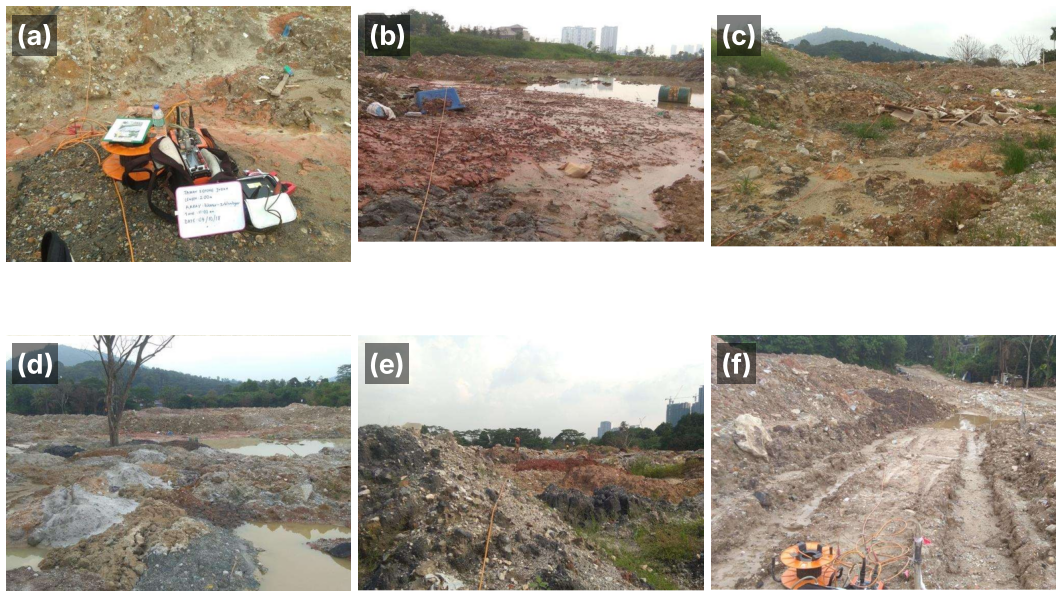
\includegraphics[width=\columnwidth]{p_fotos.png}
\caption{Condiciones del sitio: (a) equipo de adquisición, (b) charcos y residuos, (c) escombro y relleno, (d) lixiviado en depresiones, (e) cúmulo de residuos con cable de electrodos, (f) camino de acceso. Imágenes del material suplementario de \cite{arifin2020dib}.}
\label{fig:fotos}
\end{figure}

\begin{figure}[!t]
\centering
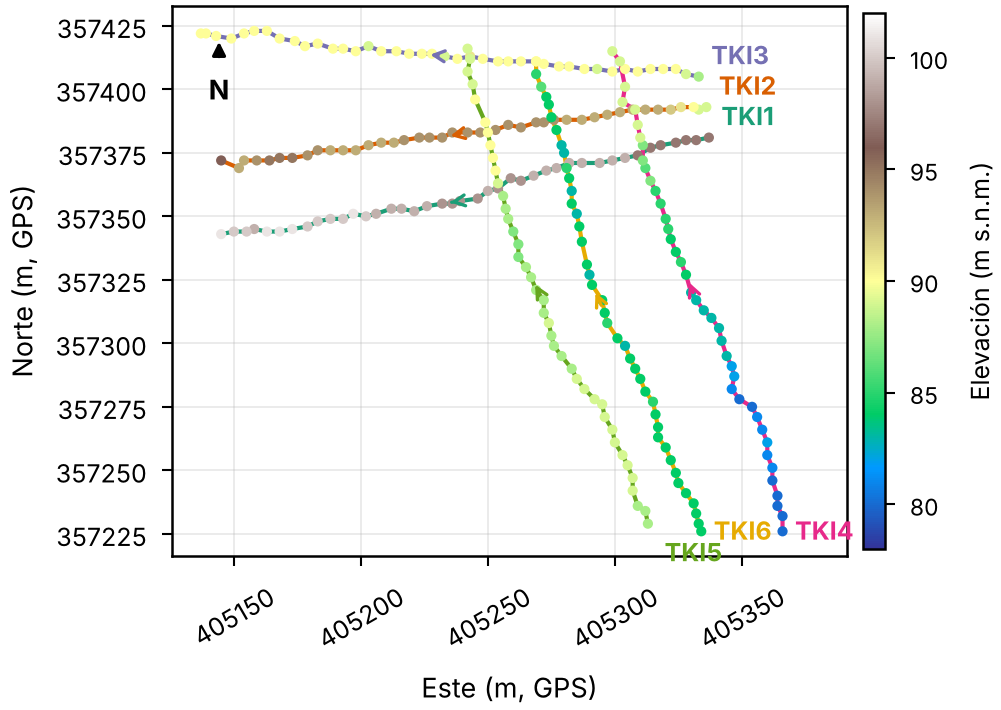
\includegraphics[width=0.92\columnwidth]{p_mapa.png}
\caption{Trazas de las seis líneas según el \gps{} de cada electrodo; el color indica la elevación y las flechas, el sentido de la distancia $x$ ($x=0$ en el extremo E para TKI1--3 y en el extremo S para TKI4--6).}
\label{fig:mapa}
\end{figure}

El artículo de referencia no describe la geología local. Por el contexto regional, es probable que el área de Kuala Lumpur--Kepong esté sobre rocas metasedimentarias del Paleozoico superior de la Formación Kenny Hill (areniscas y lutitas) \cite{tan1977,filipov2021}, y se supone que Bukit Lagong es de granito de la Cordillera Principal. Con esa suposición, la clase de resistividad $>400$\,\ohmm{} correspondería a roca poco alterada bajo una capa de suelo residual y de relleno hecho por el hombre. Es una hipótesis que debe confirmarse con la carta geológica del Departamento de Minerales y Geociencias de Malasia o con sondeos.

\section{Metodología}
\subsection{Adquisición e instrumentación}
Según \cite{arifin2020dib}, se usó un resistivímetro ABEM Terrameter SAS4000 con un selector electrónico ABEM LUND ES10-64C. Se colocaron 41 electrodos de acero inoxidable con arreglo Wenner--Schlumberger, separados 5\,m (200\,m de largo y unos 35\,m de profundidad de investigación), y se inyectó una corriente de 50 a 100\,mA. Los archivos \texttt{.dat} en formato RES2DINV contienen entre 294 y 317 mediciones por línea (1\,862 en total), con $n\le8$ y $a\le15$\,m, que describen la geometría de cada medición. La cargabilidad se registró en el dominio del tiempo (en ms), con tiempos de retardo e integración de 0.2 y 1\,023 según el encabezado de los archivos (Tabla~\ref{tab:params}).

\begin{table}[!t]
\caption{Parámetros de adquisición y de los datos}
\label{tab:params}
\centering
\small
\begin{tabular}{@{}lc@{}}
\toprule
Parámetro & Valor \\
\midrule
Arreglo / separación & Wenner--Schlumberger / 5\,m \\
Electrodos / longitud & 41 / 200\,m \\
Mediciones por línea & 294--317 \\
$\rho_a$ medida & 19--389\,\ohmm \\
IP aparente (crudo) & 0.02--134\,ms \\
Retardo / integración IP (encabezado) & 0.2 / 1\,023 \\
Cota del terreno (\gps) & 80--101\,m \\
Datos eliminados ($\rho$ / IP) & 149 / 70 adicionales \\
\bottomrule
\end{tabular}
\end{table}

\subsection{Topografía}
De cada electrodo se tenía su posición este (E), norte (N) y elevación del \gps. Con esos datos se calculó la distancia horizontal acumulada y la elevación a lo largo de cada línea, y se añadió la topografía a los archivos \texttt{.dat} (versión completa y versión editada). La malla de la inversión sigue el relieve. Las cotas \gps{} de las líneas E--O y N--S difieren hasta 14\,m donde se cruzan. Por eso el modelo 3D se construyó en profundidad bajo la superficie y no en cota absoluta.

\subsection{Edición de datos}
Se revisaron la cargabilidad aparente y el desajuste de $\rho_a$ (la diferencia entre lo medido y lo calculado) para cada electrodo de potencial (Fig.~\ref{fig:qc}). El electrodo 28 ($x=140$\,m) produjo en todas las líneas una IP aparente mediana de 10 a 30\,ms (contra 1--3\,ms en el resto) y desajustes altos. Se eliminaron además el electrodo 25 en TKI1 y el 7 en TKI3. Después de una primera inversión se descartaron los datos con desajuste mayor que $\max(25\,\mathchar"0025,\,3\sigma)$. En total se retiraron 149 mediciones para la resistividad (8\,\%; 92 por el electrodo 28, 26 por el 25, 18 por el 7 y 13 atípicas) y otras 70 solo para el modelo de IP, con un criterio robusto. Las bitácoras completas se entregan en archivos \texttt{.csv}.

\begin{figure*}[!t]
\centering
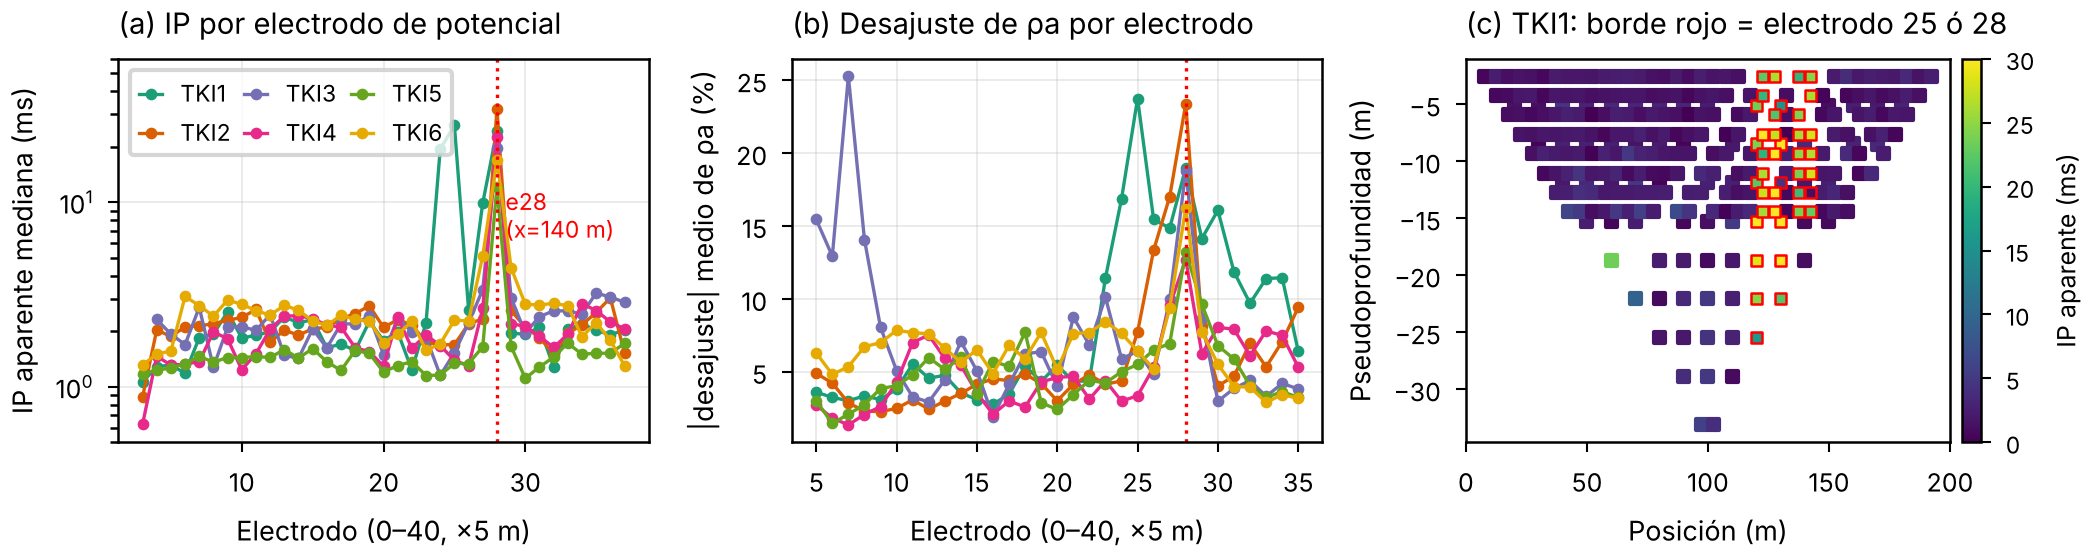
\includegraphics[width=\textwidth]{p_qc.png}
\caption{Control de calidad: (a) IP aparente mediana por electrodo de potencial, (b) desajuste medio de $\rho_a$ por electrodo y (c) pseudosección de IP de TKI1 con las mediciones de los electrodos 25 y 28 (borde rojo).}
\label{fig:qc}
\end{figure*}

\subsection{Inversión de resistividad}
La inversión es el proceso matemático que convierte las mediciones en un modelo del subsuelo. No se contó con RES2DINV, el programa que usó \cite{arifin2020dib}. Por eso se programó en Python un código propio con la misma formulación general: un modelado directo 2.5D por elementos finitos \cite{dey1979} sobre una malla que sigue la topografía, y una inversión por mínimos cuadrados con restricción de suavidad \cite{degroot1990,loke1996}, resuelta con el método de Gauss--Newton:
\begin{equation}
\left(\mathbf{J}^{T}\mathbf{J}+\lambda\,\mathbf{C}^{T}\mathbf{C}\right)\Delta\mathbf{m}=\mathbf{J}^{T}\mathbf{d}-\lambda\,\mathbf{C}^{T}\mathbf{C}\,\mathbf{m},
\label{eq:gn}
\end{equation}
donde $\mathbf{m}=\ln\rho$ es el modelo (el logaritmo de la resistividad), $\mathbf{d}=\ln\rho_a^{\mathrm{obs}}-\ln\rho_a^{\mathrm{calc}}$ es la diferencia entre lo observado y lo calculado, $\mathbf{J}$ es la matriz de sensibilidad (cuánto cambia cada medición si cambia cada celda), $\mathbf{C}$ es el operador de suavidad y $\lambda$ es el factor de amortiguamiento. El error se expresa como RMS relativo de $\rho_a$, en porcentaje. Los resultados no son idénticos a los de RES2DINV; los archivos \texttt{.dat} con topografía permiten repetir el proceso en ese programa \cite{loke2016}.

\subsection{Selección de la iteración}
Se hicieron 10 iteraciones por línea (Fig.~\ref{fig:iter}). Se eligió la iteración 4 en todas, por tres razones: (i) el RMS ya varía menos de 5\,\% respecto de la iteración anterior (3.4 a 4.9\,\%); (ii) la resistividad máxima del modelo es del orden del máximo de 2\,000\,\ohmm{} de la clase de basamento del artículo (214 a 1\,763\,\ohmm{} en las celdas de la inversión; 251 a 2\,040\,\ohmm{} en los modelos interpolados de la Tabla~\ref{tab:zonas}); y (iii) no es menor que el 95\,\% de la $\rho_a$ máxima medida. Después de la iteración 4, la resistividad máxima de TKI6 oscila entre $1.7\times10^{3}$ y $10^{4}$\,\ohmm{} mientras el RMS solo baja de 7.4 a 5.5\,\%, lo que sugiere que el modelo se ajusta al ruido.

\begin{figure*}[!t]
\centering
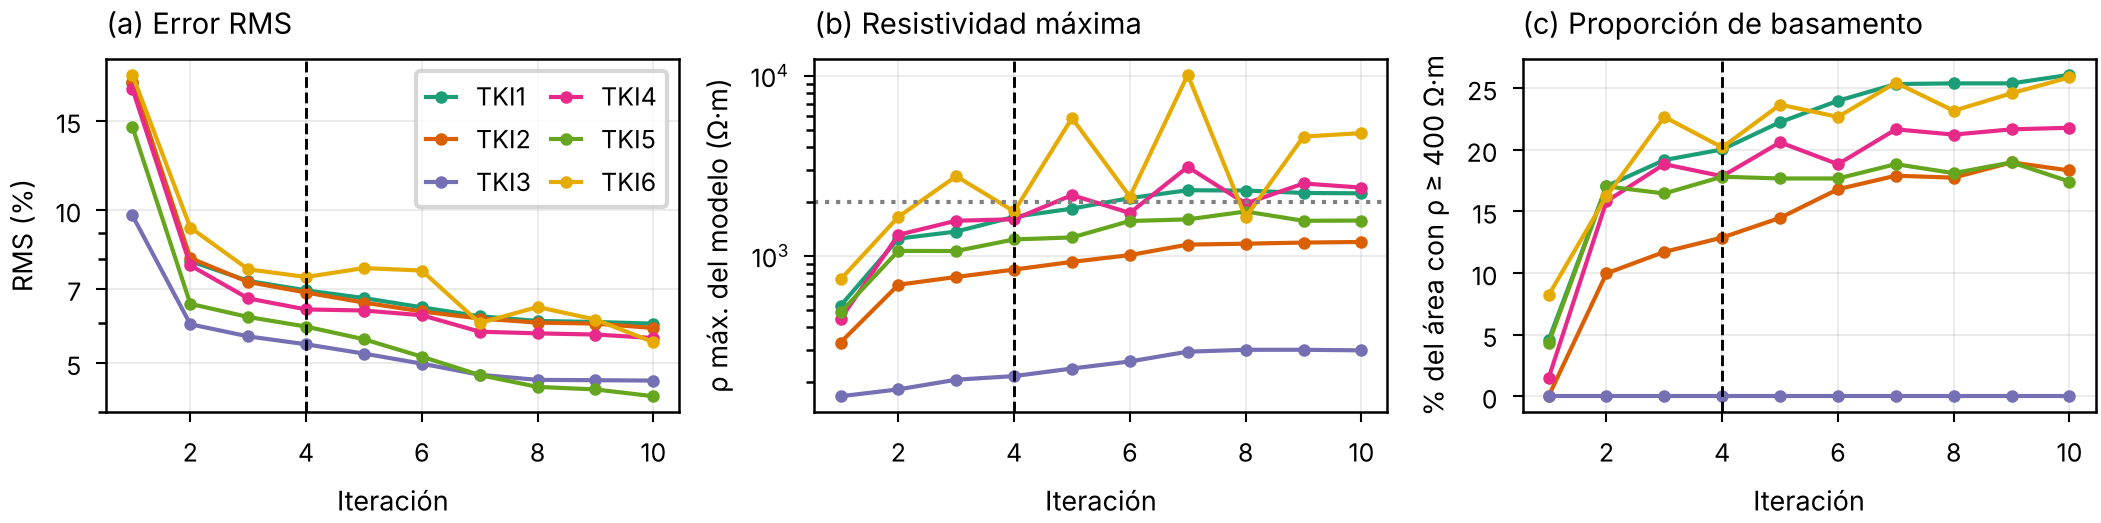
\includegraphics[width=\textwidth]{p_iter.png}
\caption{Efecto del número de iteraciones: (a) RMS, (b) resistividad máxima del modelo (línea punteada: 2\,000\,\ohmm, máximo del artículo) y (c) proporción del área con $\rho\ge400$\,\ohmm. La línea discontinua marca la iteración elegida (4).}
\label{fig:iter}
\end{figure*}

\subsection{Modelo de cargabilidad}
La cargabilidad se invirtió de forma lineal sobre el modelo final de resistividad, con la relación de Seigel \cite{seigel1959}, $m_{a,i}=\sum_j S_{ij}\,m_j$ con $S_{ij}=\partial\ln\rho_{a,i}/\partial\ln\rho_j$, con suavidad y con cotas para que los valores no sean negativos \cite{oldenburg1994}. El error se reporta en ms absolutos (0.60 a 0.92\,ms).

\subsection{Modelo 3D y volumen}
Las seis secciones se muestrearon cada 1\,m en horizontal y 0.5\,m en vertical, se georreferenciaron con el \gps{} y se interpolaron a una malla de $5\times5\times1$\,m. La interpolación pondera cada dato por el inverso de su distancia (una distancia anisótropa en E, N y profundidad), con radio de 45\,m en horizontal y 2\,m en vertical. Solo se interpolan las celdas a menos de 45\,m de algún perfil. Los volúmenes se obtienen contando celdas de 25\,\mcub, y las isosuperficies, con el algoritmo \textit{marching cubes}. Este procedimiento sustituye a Voxler y Oasis Montaj, y los datos se exportan en formato \texttt{.vtk} y \texttt{.csv} para esos programas y para ParaView.

\section{Resultados y discusión}
\subsection{Ajuste y modelos 2D de resistividad}
El RMS en la iteración elegida es de 6.9, 6.9, 5.4, 6.4, 5.9 y 7.4\,\% para TKI1 a TKI6 (Tabla~\ref{tab:zonas}). La Fig.~\ref{fig:pseudo} compara las pseudosecciones medida y calculada de TKI1 con su modelo. Todos los modelos usan la misma escala logarítmica de 5 a 4\,000\,\ohmm{} (Fig.~\ref{fig:seisrho}).

\begin{figure}[!t]
\centering
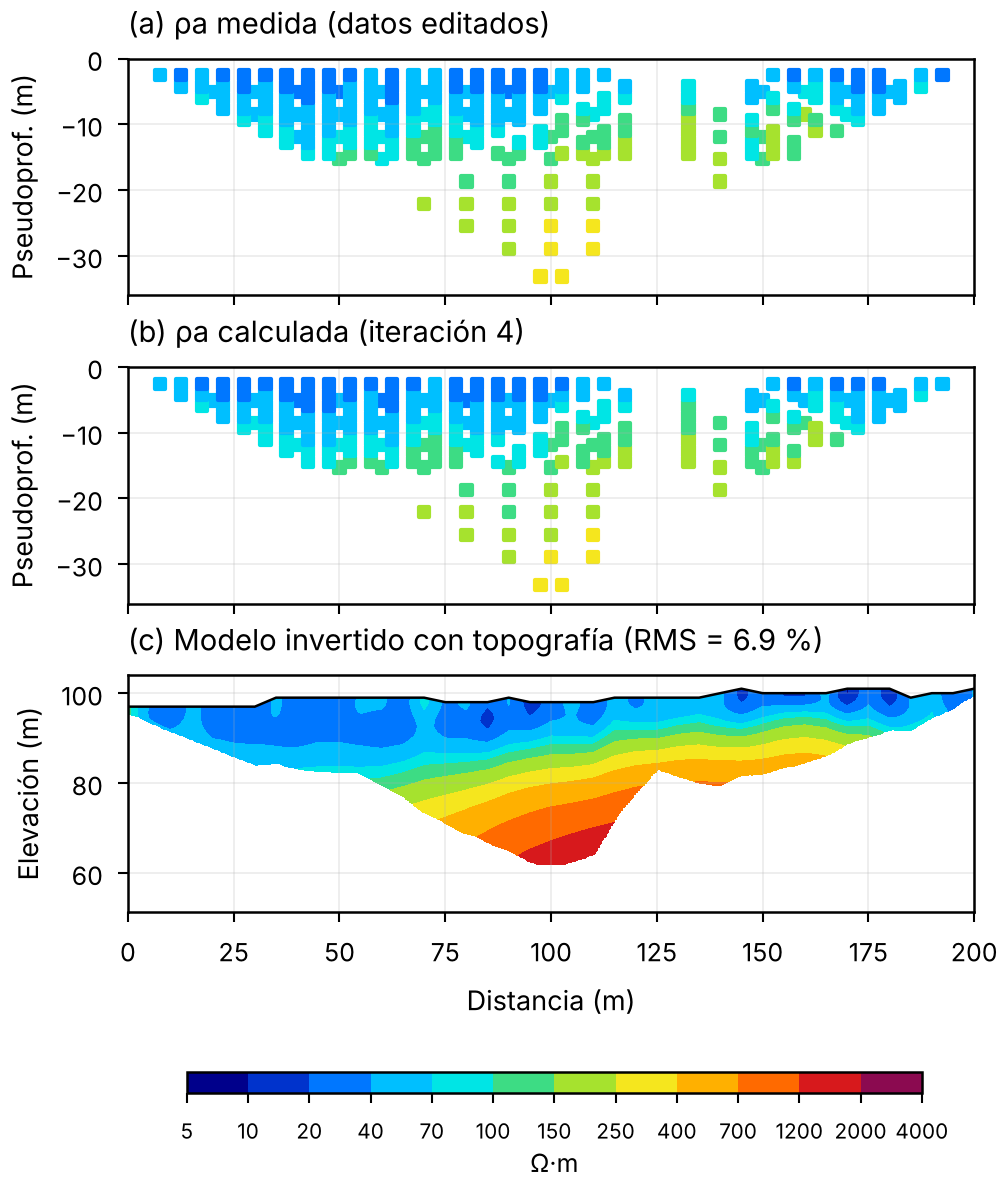
\includegraphics[width=0.92\columnwidth]{p_pseudo_TKI1.png}
\caption{TKI1: (a) pseudosección medida (datos editados), (b) calculada en la iteración 4 y (c) modelo invertido con topografía. El vacío en $x\approx120$--$135$\,m resulta de eliminar el electrodo 28.}
\label{fig:pseudo}
\end{figure}

Siguiendo la clasificación de \cite{arifin2020dib} se marcaron tres zonas con isolíneas de 100\,\ohmm{} (continua) y 400\,\ohmm{} (discontinua), y el núcleo más afectado con $\rho<30$\,\ohmm{} (magenta):
\begin{itemize}
\item \textbf{Capa blanda / residuos} ($<100$\,\ohmm): ocupa del 43 al 82\,\% de cada sección. Su base media está a 8.4\,m en TKI5, 9.6\,m en TKI1, 11.2\,m en TKI2, 13.0\,m en TKI4 y TKI6, y 18.8\,m en TKI3; la base máxima llega a 14.9--21.4\,m. La resistividad mediana es de 39\,\ohmm{} (P10--P90: 23--74\,\ohmm, es decir, el 80\,\% central de los valores).
\item \textbf{Capa consolidada} (100--400\,\ohmm): es una banda de transición, bien desarrollada en TKI5 (40\,\% del área) y TKI2 (28\,\%).
\item \textbf{Basamento} ($>400$\,\ohmm): aparece entre $x\approx62$ y 165\,m, bajo la parte central de TKI1, TKI2, TKI4, TKI5 y TKI6. Su techo está a 13.5--19.0\,m en el punto más somero, a 17.3--21.7\,m en promedio y hasta a 31\,m. En TKI3 la resistividad máxima es de 251\,\ohmm: no se llega a la clase de basamento en los 35\,m de investigación.
\end{itemize}
La Fig.~\ref{fig:tki5} muestra el ejemplo anotado de TKI5, y la Tabla~\ref{tab:zonas} resume las seis líneas.

\begin{figure*}[!t]
\centering
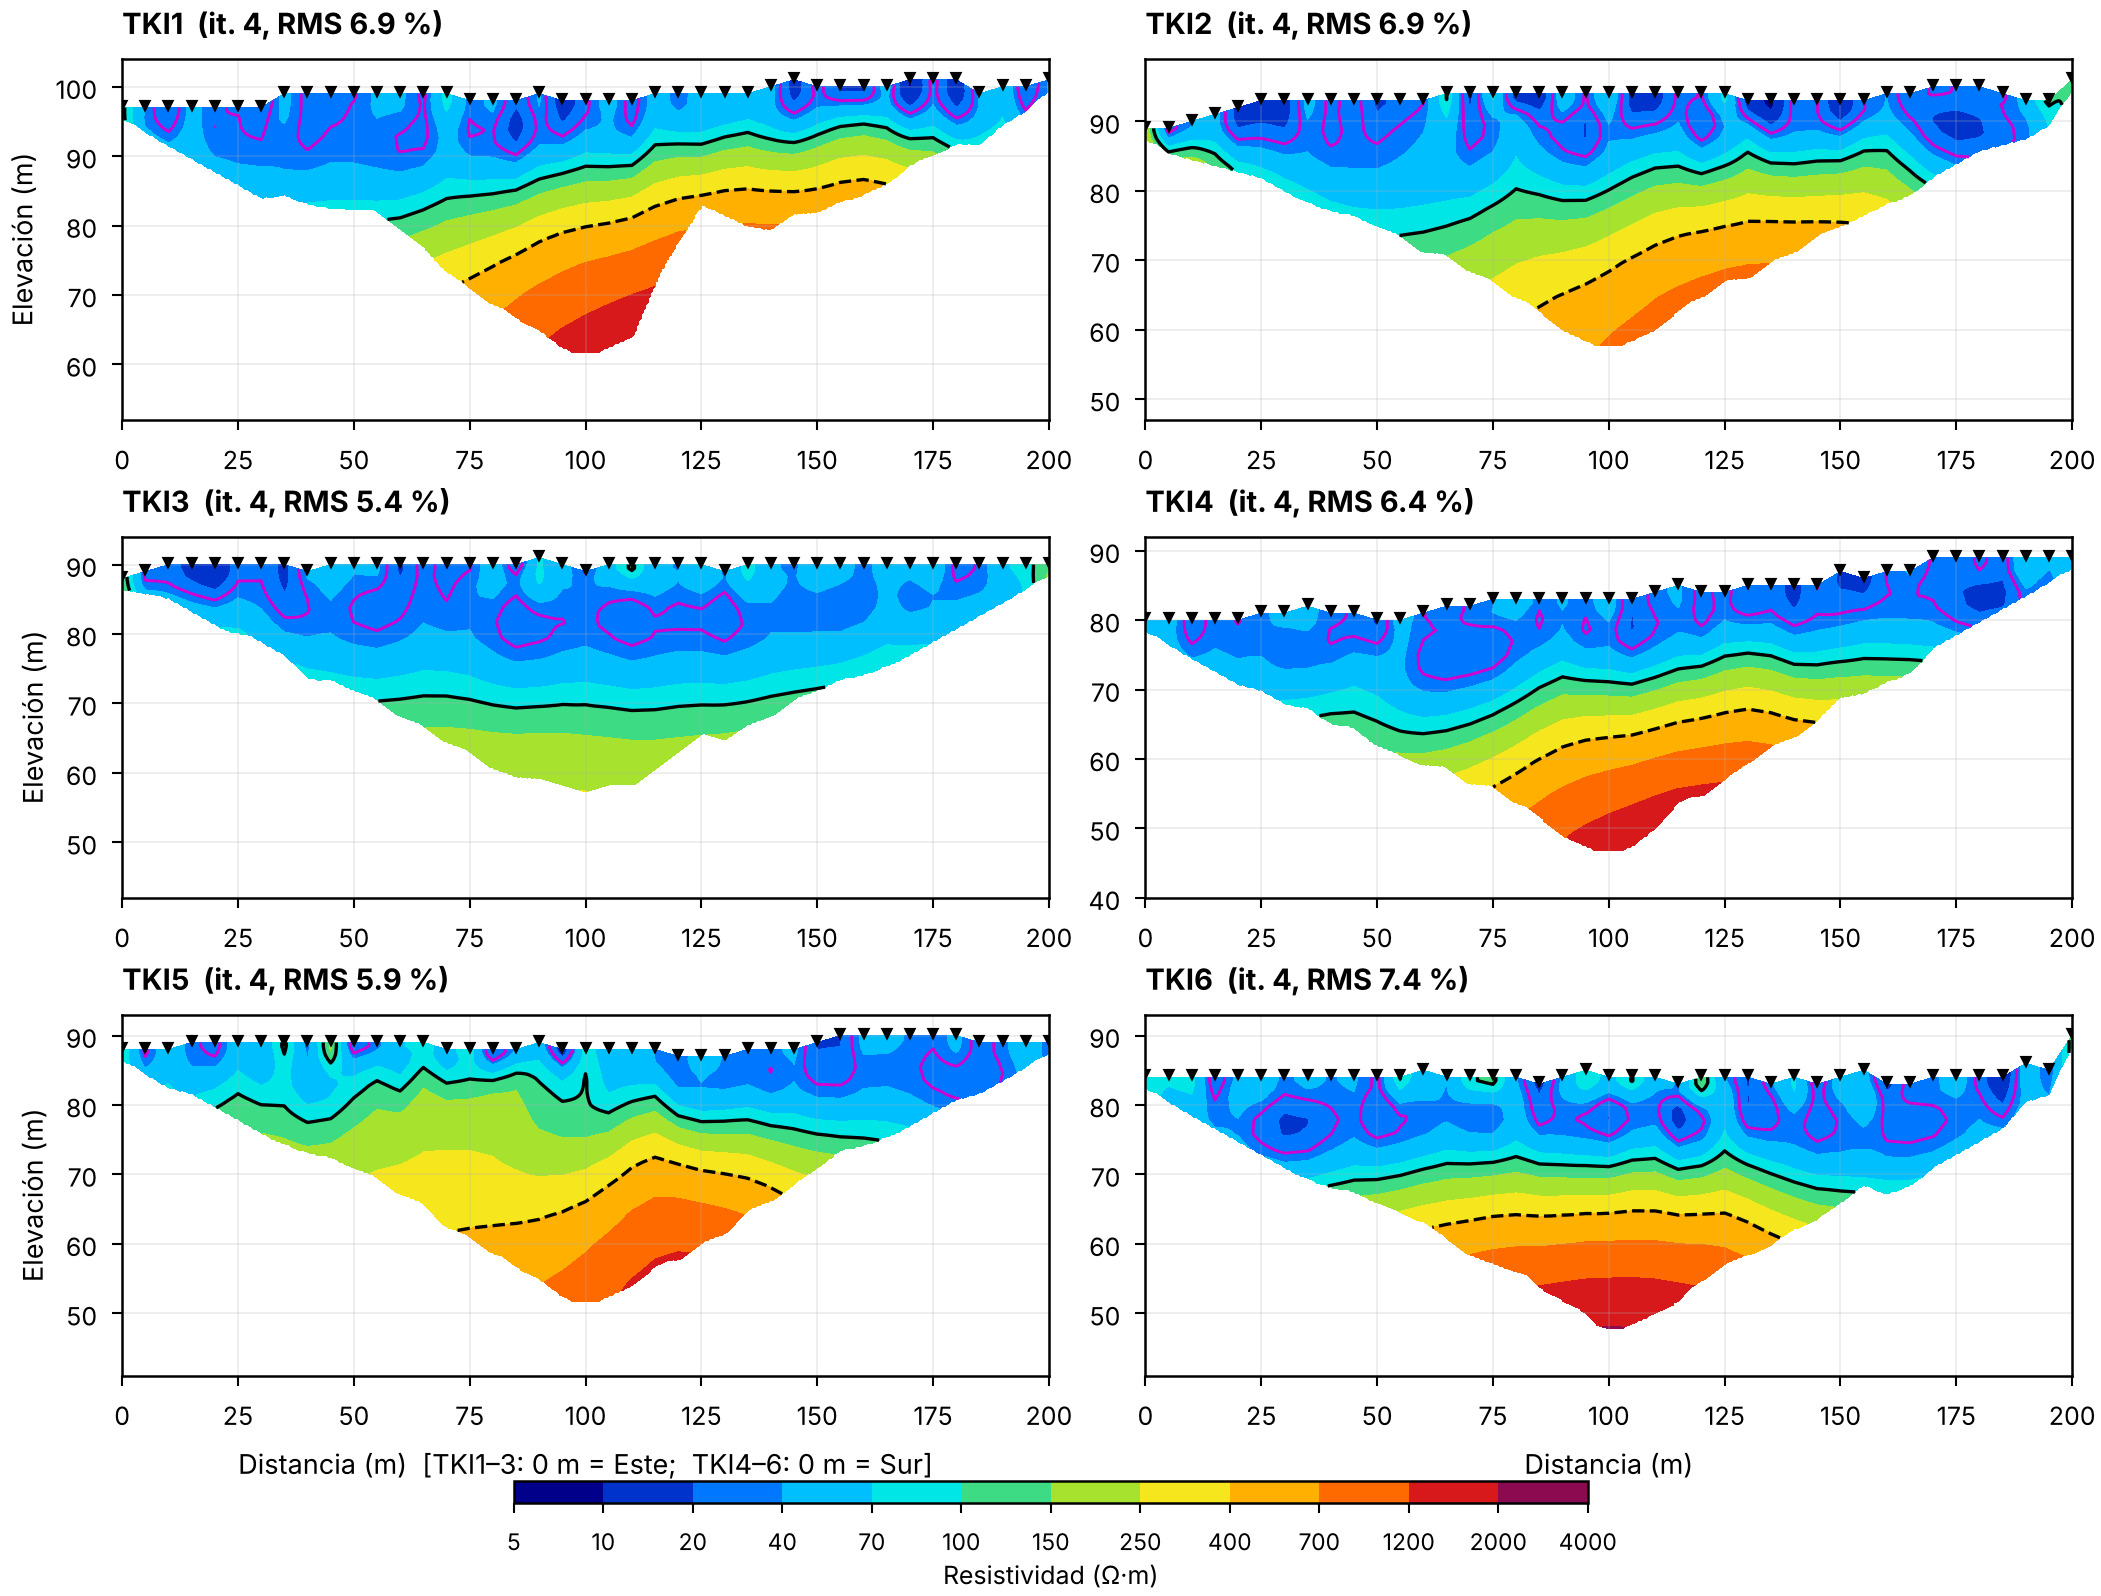
\includegraphics[width=\textwidth]{p_seis_rho.png}
\caption{Modelos de resistividad de las seis líneas (iteración 4, misma escala). Isolíneas: 100\,\ohmm{} (continua), 400\,\ohmm{} (discontinua) y 30\,\ohmm{} (magenta). Triángulos: electrodos. Para TKI1--3 $x=0$ es el extremo E; para TKI4--6, el extremo S.}
\label{fig:seisrho}
\end{figure*}

\begin{figure*}[!t]
\centering
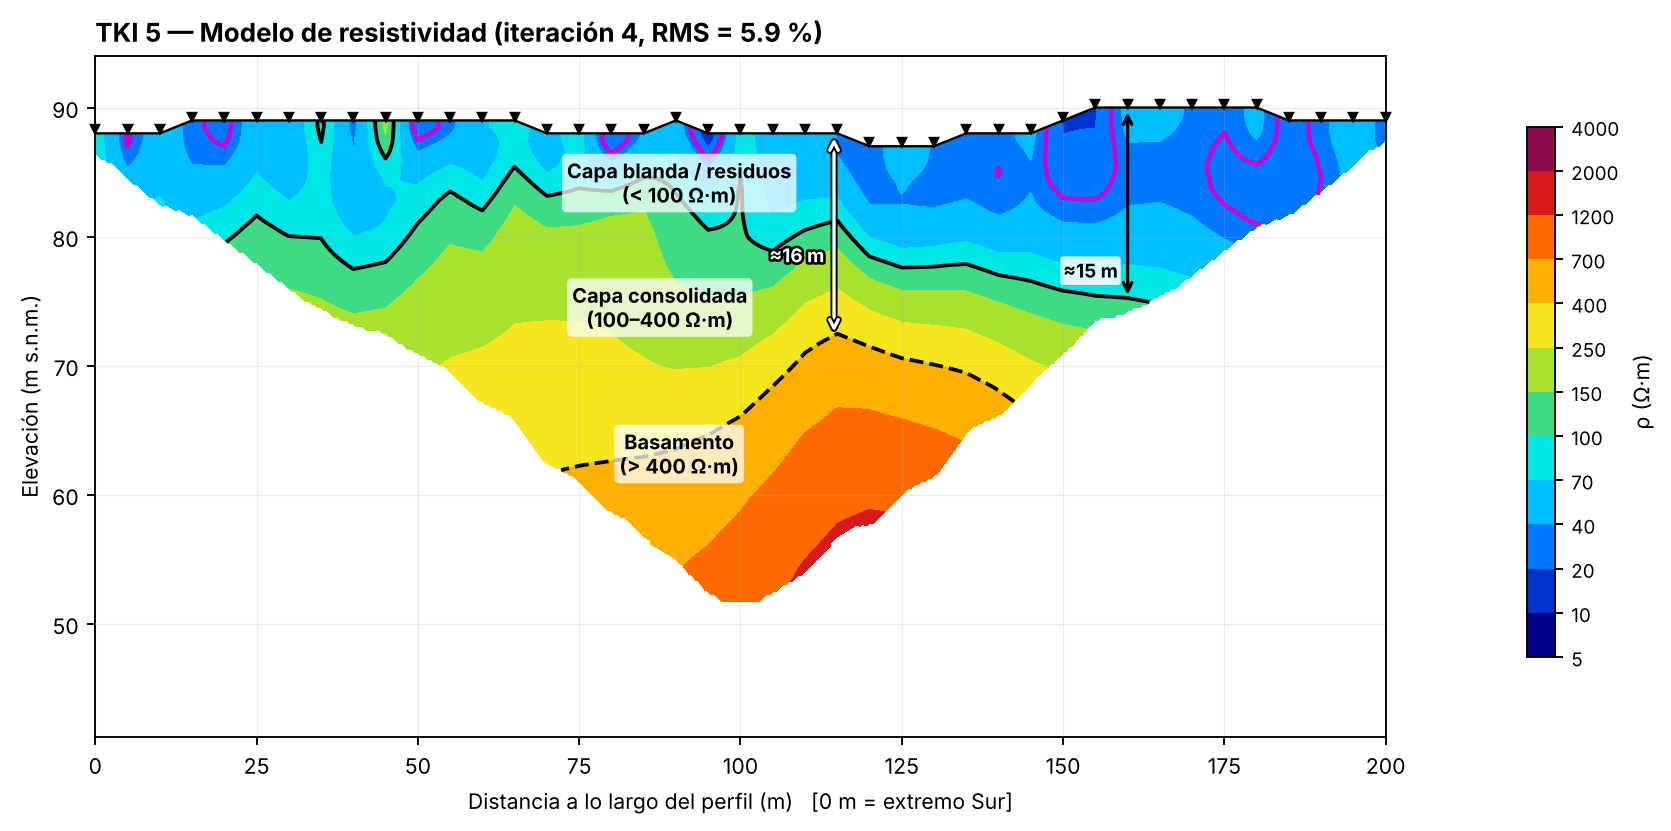
\includegraphics[width=0.94\textwidth]{p_TKI5_anotado.png}
\caption{TKI5 con las zonas anotadas: capa blanda/residuos, capa consolidada y basamento, con la profundidad aproximada al techo del basamento ($\approx16$\,m en $x\approx115$\,m) y el espesor aproximado de la capa blanda ($\approx15$\,m en $x\approx160$\,m).}
\label{fig:tki5}
\end{figure*}

\begin{table*}[!t]
\caption{Resumen por línea (iteración 4). Porcentajes de área de la sección; profundidades bajo la superficie}
\label{tab:zonas}
\centering
\small
\begin{tabular}{@{}lcccccc@{}}
\toprule
Línea & \thead{RMS\\(\%)} & \thead{$\rho$ mín--máx\\(\ohmm)} & \thead{Blanda / consol. / basam.\\(\% del área)} & \thead{Base de la blanda\\media / máx. (m)} & \thead{Techo del basamento\\mín / media / máx. (m)} & \thead{Núcleo $<30$\,\ohmm\\m\textsuperscript{2} (\%)} \\
\midrule
TKI1 & 6.9 & 9--1\,706 & 55 / 25 / 20 & 9.6 / 18.1 & 13.5 / 17.3 / 26.5 & 362 (10) \\
TKI2 & 6.9 & 8--866 & 59 / 28 / 13 & 11.2 / 19.4 & 17.5 / 21.7 / 31.0 & 605 (16) \\
TKI3 & 5.4 & 10--251 & 82 / 18 / 0 & 18.8 / 21.4 & -- & 460 (12) \\
TKI4 & 6.4 & 15--1\,829 & 60 / 22 / 18 & 13.0 / 17.9 & 17.5 / 20.3 / 27.0 & 582 (15) \\
TKI5 & 5.9 & 14--1\,266 & 43 / 40 / 18 & 8.4 / 14.9 & 15.8 / 20.6 / 26.2 & 184 (5) \\
TKI6 & 7.4 & 11--2\,040 & 62 / 20 / 19 & 13.0 / 16.9 & 19.0 / 20.2 / 22.5 & 480 (13) \\
\bottomrule
\end{tabular}
\end{table*}

\textbf{Ubicación y tamaño de las zonas afectadas.} Se toma como zona afectada la capa blanda y, dentro de ella, el núcleo de $\rho<30$\,\ohmm{} (las posiciones $x$ se miden desde el extremo E en TKI1--3 y desde el extremo S en TKI4--6). En TKI1 los núcleos están en $x=38$--50\,m y $x=80$--89\,m (hasta 8\,m de profundidad). En TKI2 están en $x=162$--188\,m (10\,m de espesor, el mayor), 78--98, 17--33, 47--60, 103--114 y 128--139\,m. En TKI3, en $x=5$--40, 49--64, 81--96 y 103--134\,m (hasta 12\,m). En TKI4, en $x=127$--161, 167--189, 59--79 y 102--111\,m (6 a 11\,m). En TKI5, solo en $x=148$--158 y 172--190\,m (7 a 9\,m). Y en TKI6, en $x=24$--42, 47--56, 111--121, 128--137 y 158--173\,m (7 a 11\,m). Los núcleos son someros (menos de 12\,m), miden de 8 a 35\,m de ancho y suman de 5 a 16\,\% de cada sección.

\textbf{Comparación con el artículo.} El artículo reporta una capa blanda de 10 a 15\,m, una consolidada de 15 a 20\,m y un basamento de 20 a 35\,m \cite{arifin2020dib}. La base media de la capa blanda (8--19\,m) y el techo medio del basamento (17--22\,m) caen dentro de esos intervalos, con dos diferencias: TKI3 no tiene basamento a la profundidad investigada, y en TKI1 y TKI5 el basamento llega a 13.5 y 15.8\,m, más somero que lo reportado. La línea TKI5, que el artículo señala como el peor escenario por el escurrimiento superficial, tiene la capa blanda más delgada (8.4\,m) y el núcleo más pequeño (5\,\%). Esto indica que la imagen eléctrica ve el volumen del relleno y no el lixiviado que se ve en la superficie.

\subsection{Modelo 3D}
La Fig.~\ref{fig:cercas} une las seis secciones georreferenciadas en un diagrama de cercas. Las Figs.~\ref{fig:cortes} a \ref{fig:espesor} muestran cortes horizontales, isosuperficies (superficies que encierran los volúmenes con un mismo valor) y mapas derivados.

\begin{figure*}[!t]
\centering
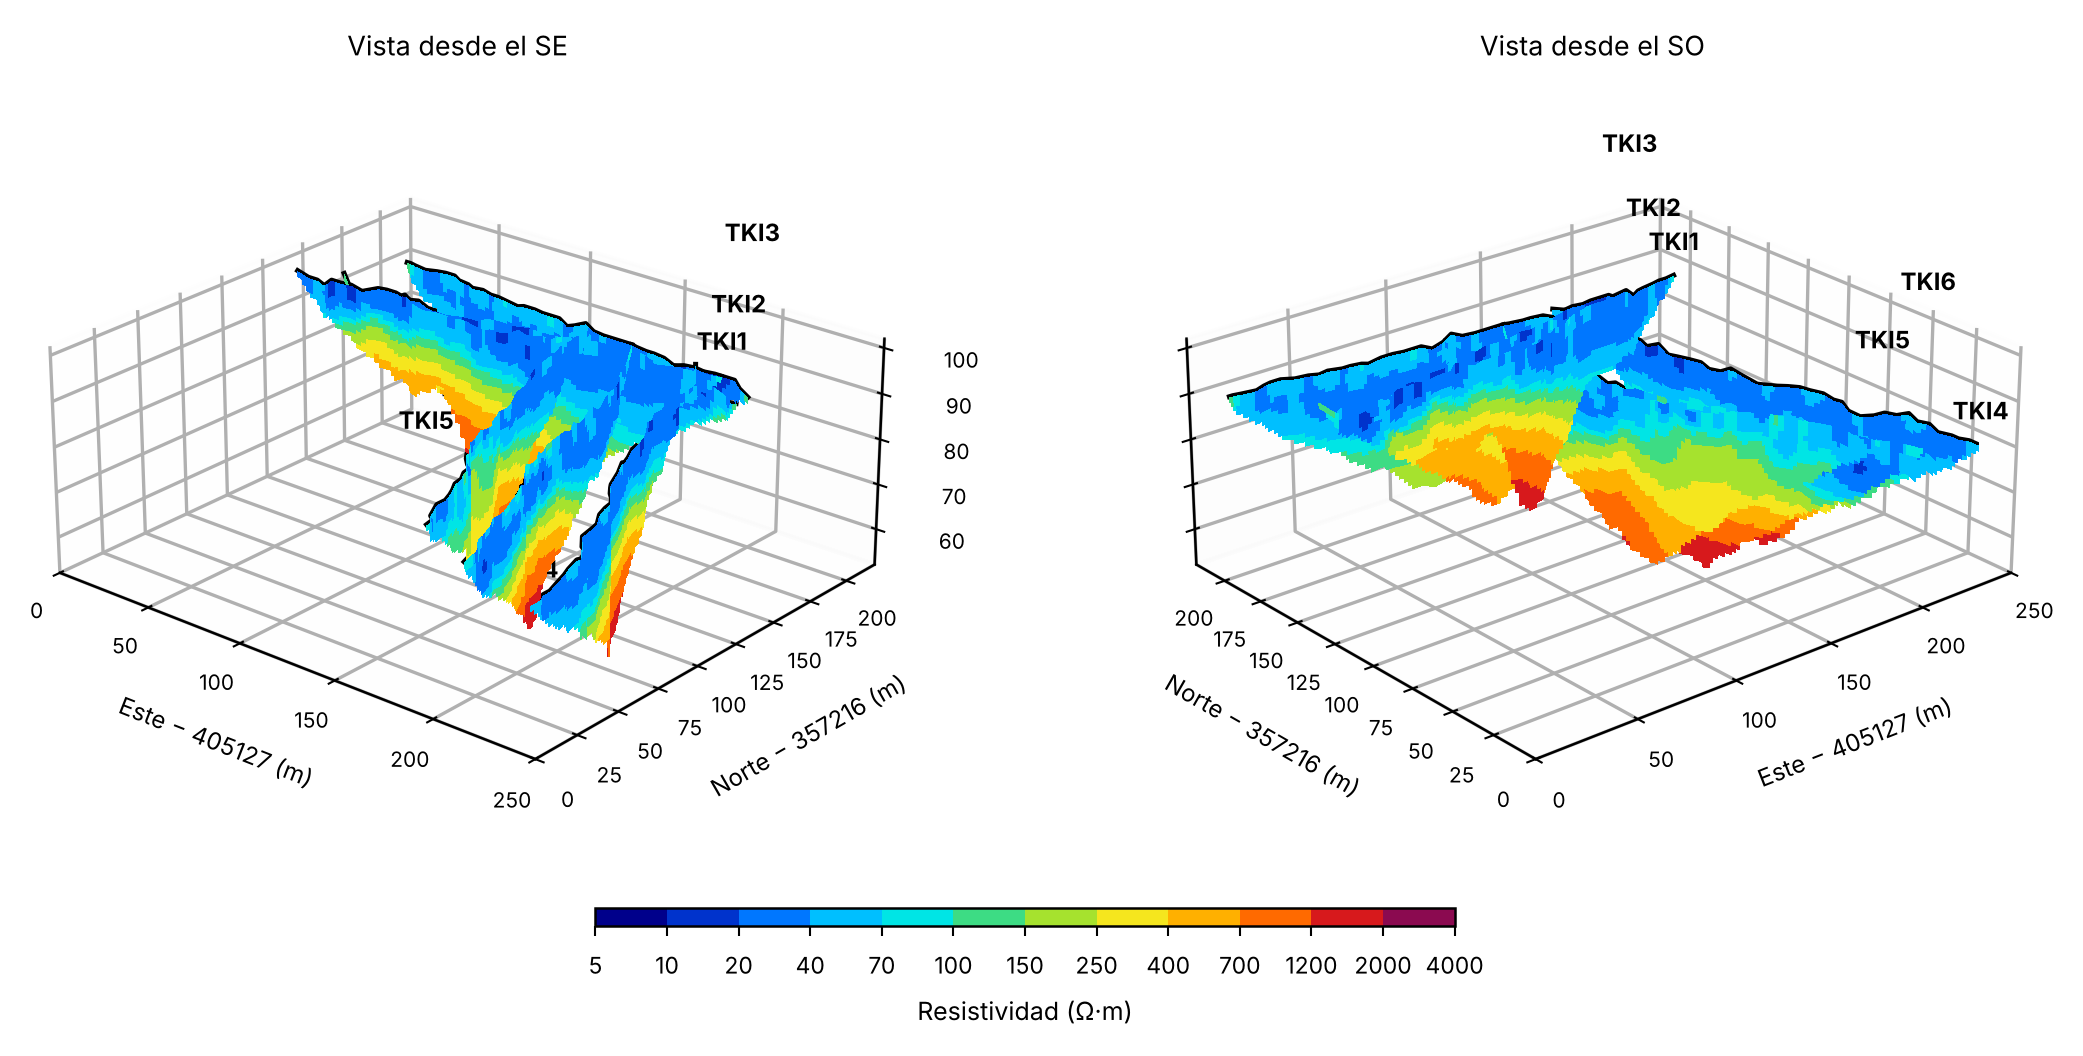
\includegraphics[width=\textwidth]{p_cercas_rho.png}
\caption{Diagrama de cercas de resistividad de las seis secciones (exageración vertical $\times2$; el eje vertical es la elevación en m s.n.m.), vistas desde el SE y el SO.}
\label{fig:cercas}
\end{figure*}

\begin{figure*}[!t]
\centering
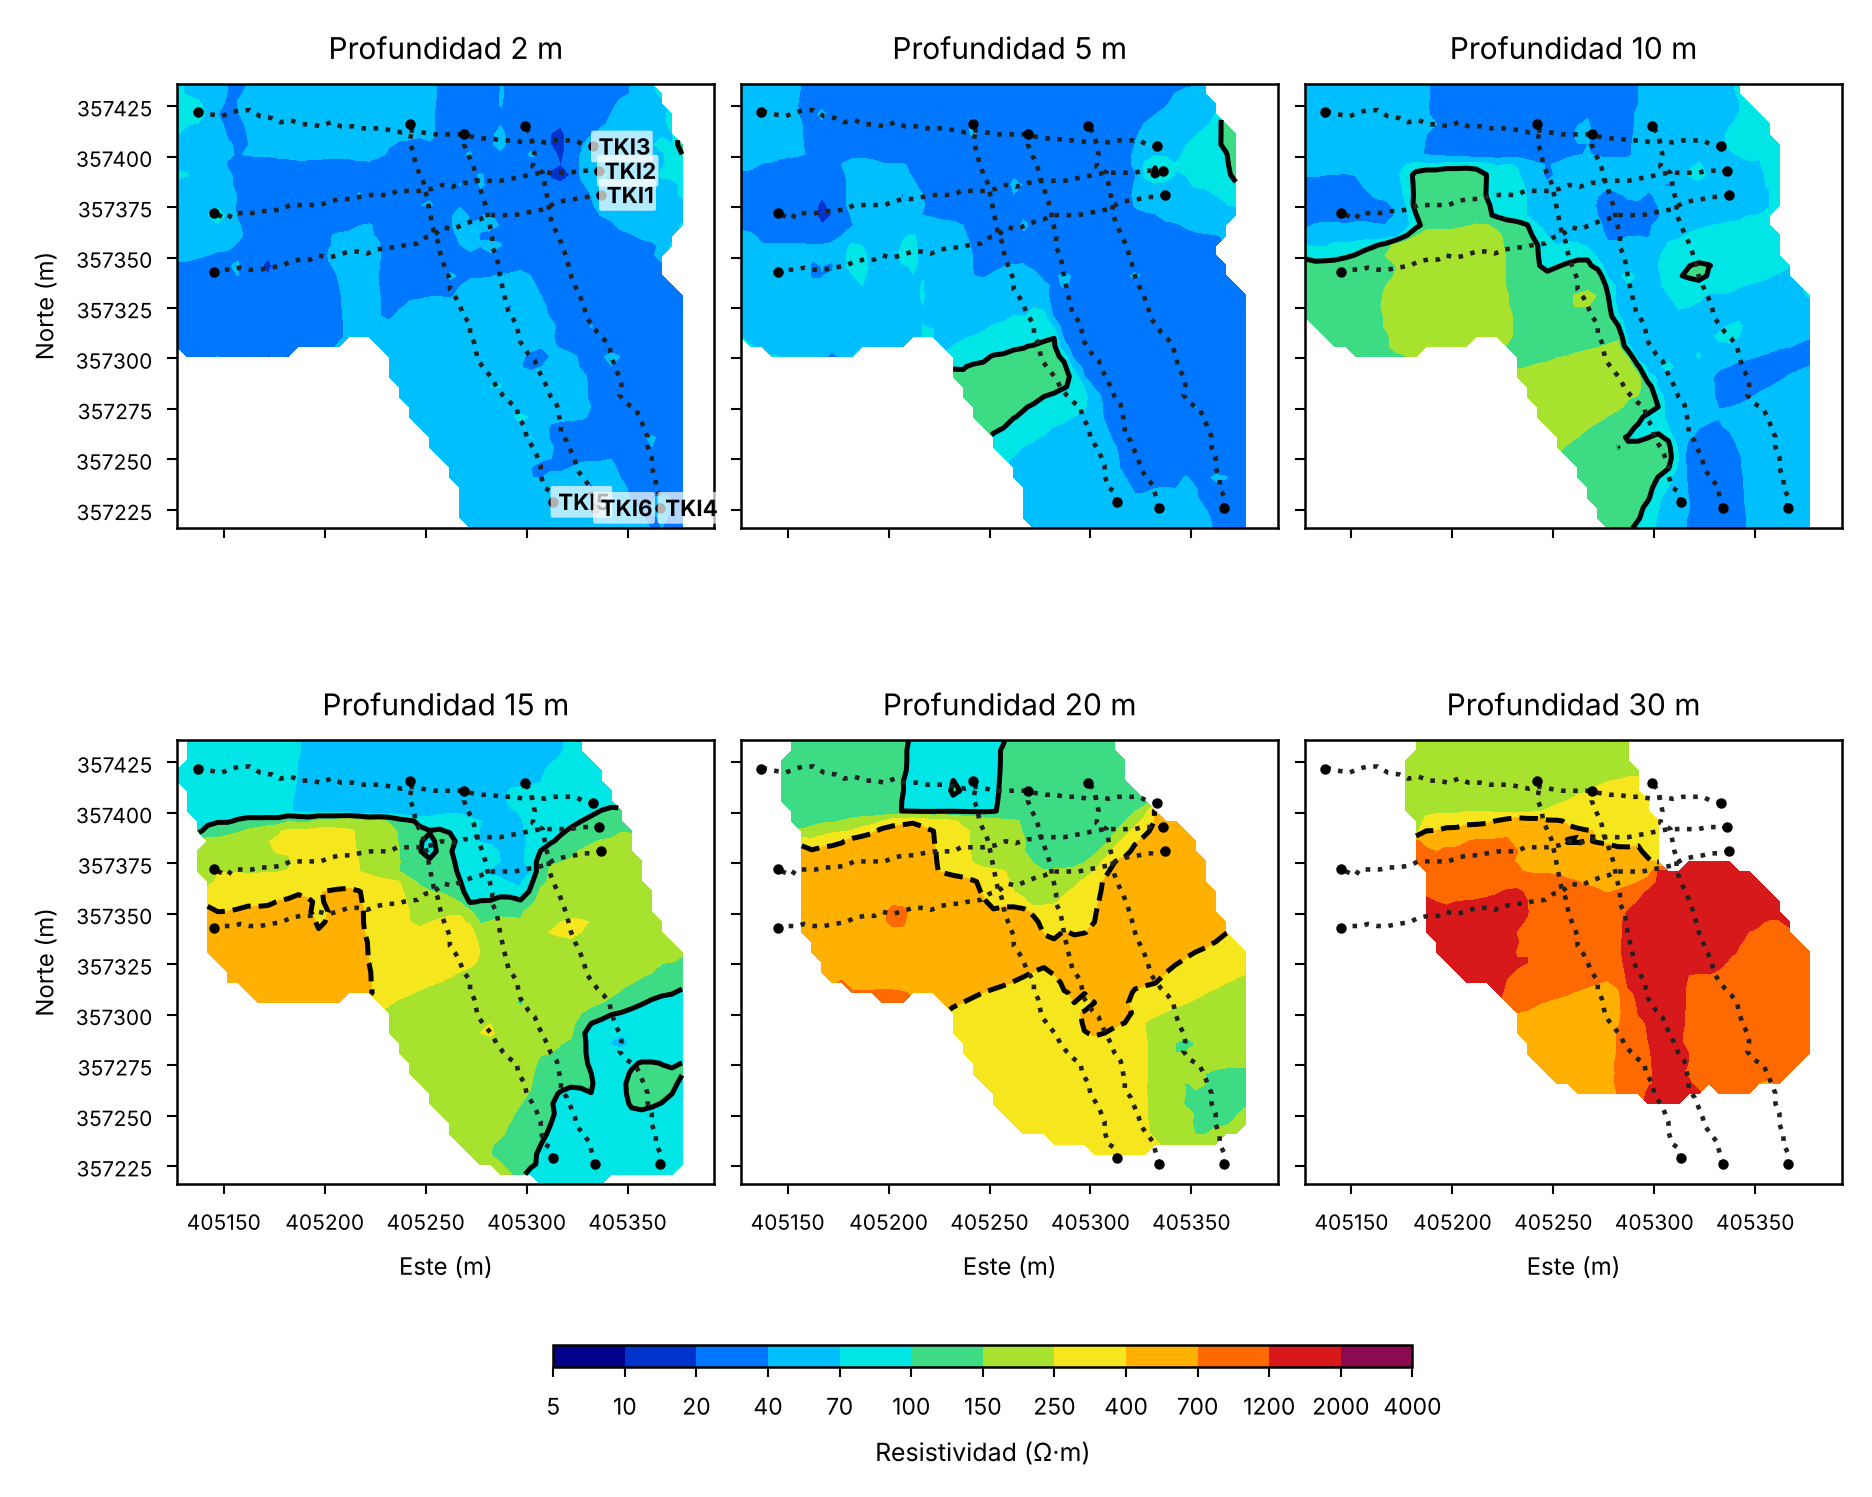
\includegraphics[width=0.94\textwidth]{p_cortes_rho.png}
\caption{Cortes horizontales de resistividad a 2, 5, 10, 15, 20 y 30\,m bajo la superficie (línea continua: 100\,\ohmm; discontinua: 400\,\ohmm). Líneas punteadas: trazas de los perfiles.}
\label{fig:cortes}
\end{figure*}

A 2\,m de profundidad todo el sitio tiene $\rho<100$\,\ohmm{} (zona afectada), con valores de 10 a 40\,\ohmm{} en el centro y el norte. A 5\,m solo dos pequeñas zonas, en el suroeste y el noreste, superan 100\,\ohmm. A 10\,m aparece resistividad de 100 a 250\,\ohmm{} en el oeste y el centro (el techo de la capa consolidada). A 15 y 20\,m la clase consolidada cubre la mayor parte del área y el contorno de 400\,\ohmm{} avanza desde el oeste. A 30\,m predominan los valores de 700 a 2\,000\,\ohmm. El norte (cerca de TKI3) se mantiene por debajo de 150\,\ohmm{} hasta los 20\,m y por debajo de 250\,\ohmm{} a 30\,m.

\begin{figure*}[!t]
\centering
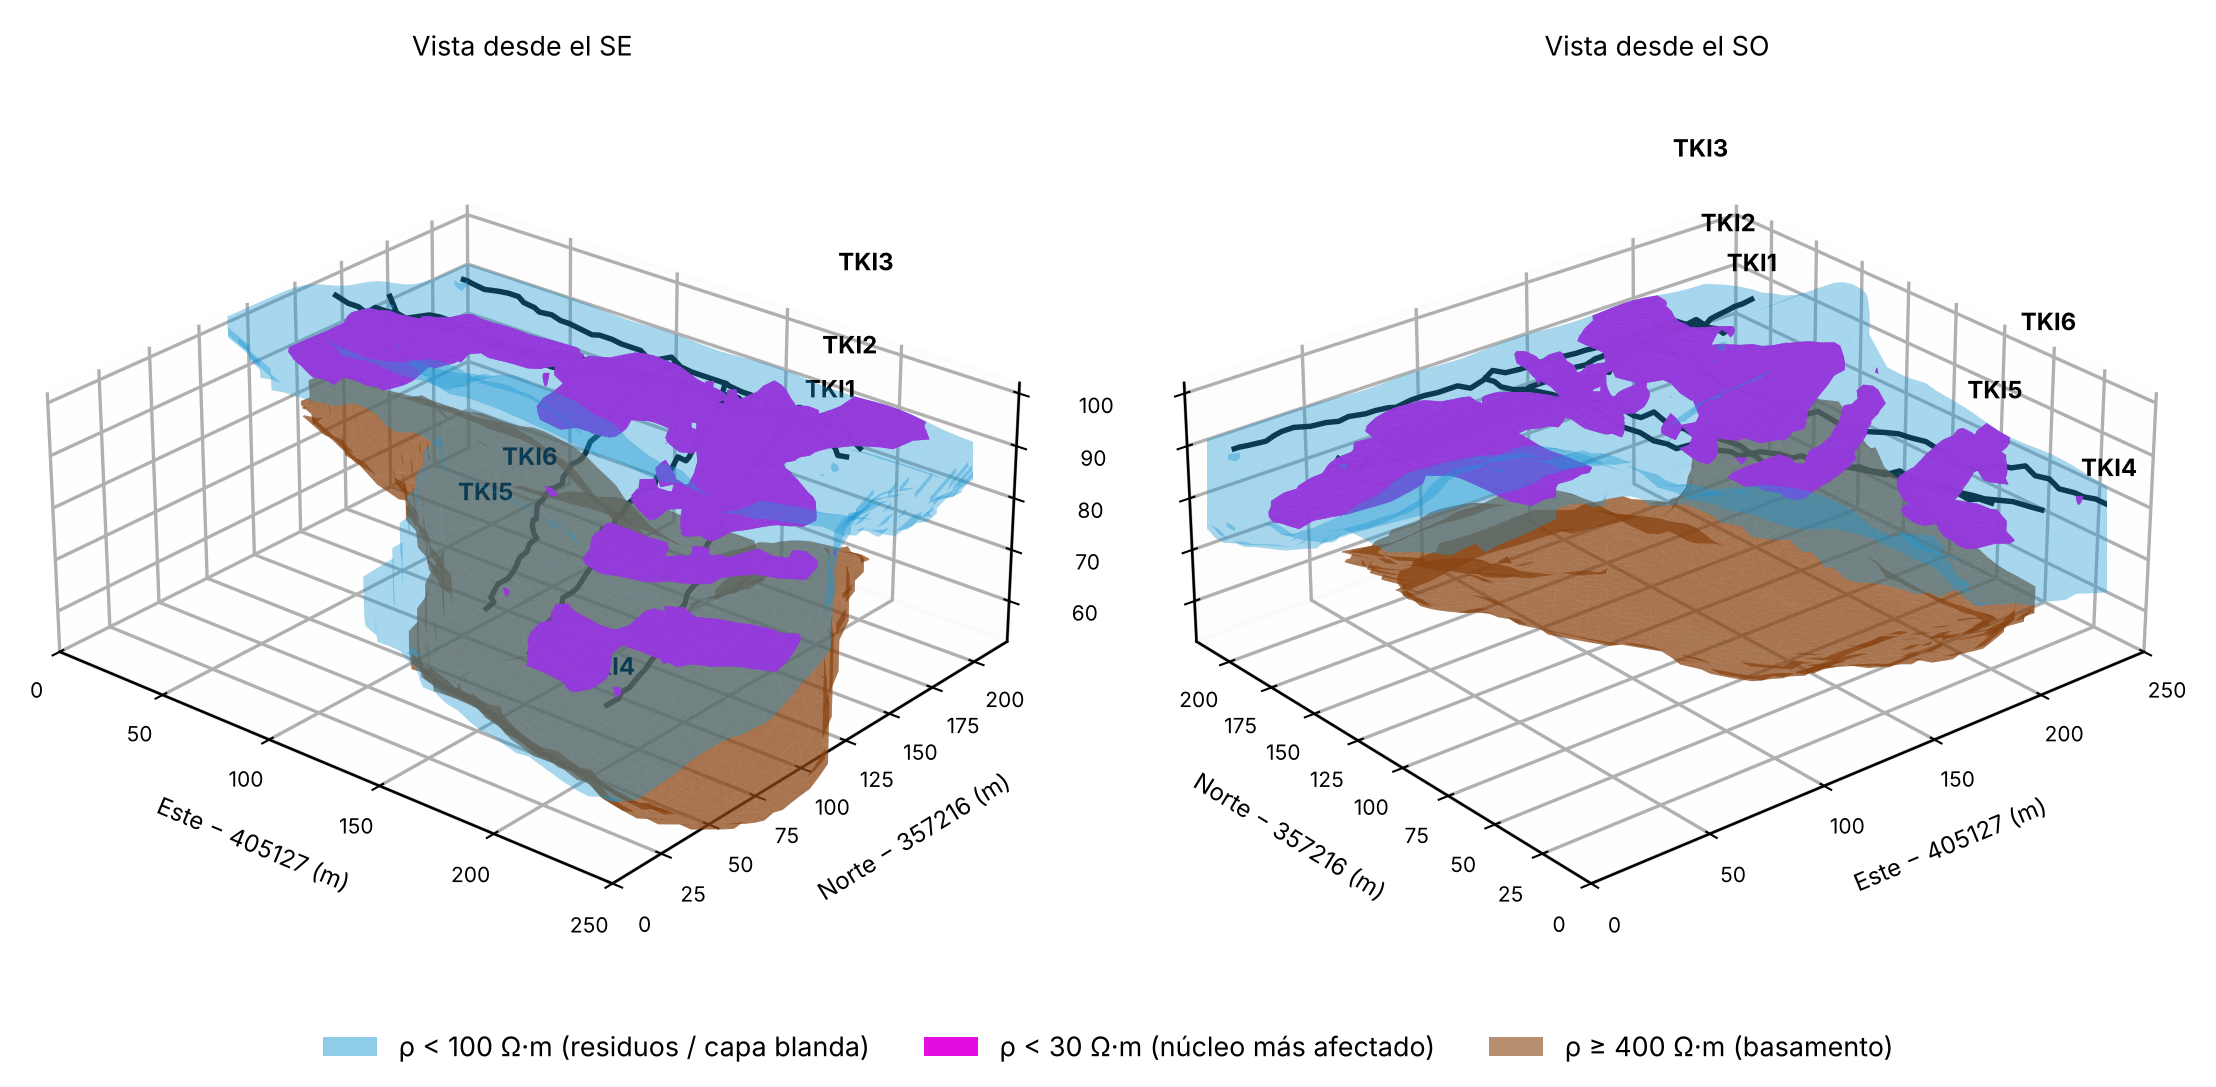
\includegraphics[width=\textwidth]{p_iso.png}
\caption{Isosuperficies de resistividad: $<100$\,\ohmm{} (azul claro, residuos/capa blanda), $<30$\,\ohmm{} (violeta, núcleo más afectado) y $\ge400$\,\ohmm{} (café, basamento). Eje vertical: elevación en m s.n.m., exageración $\times2$.}
\label{fig:iso}
\end{figure*}

\begin{figure*}[!t]
\centering
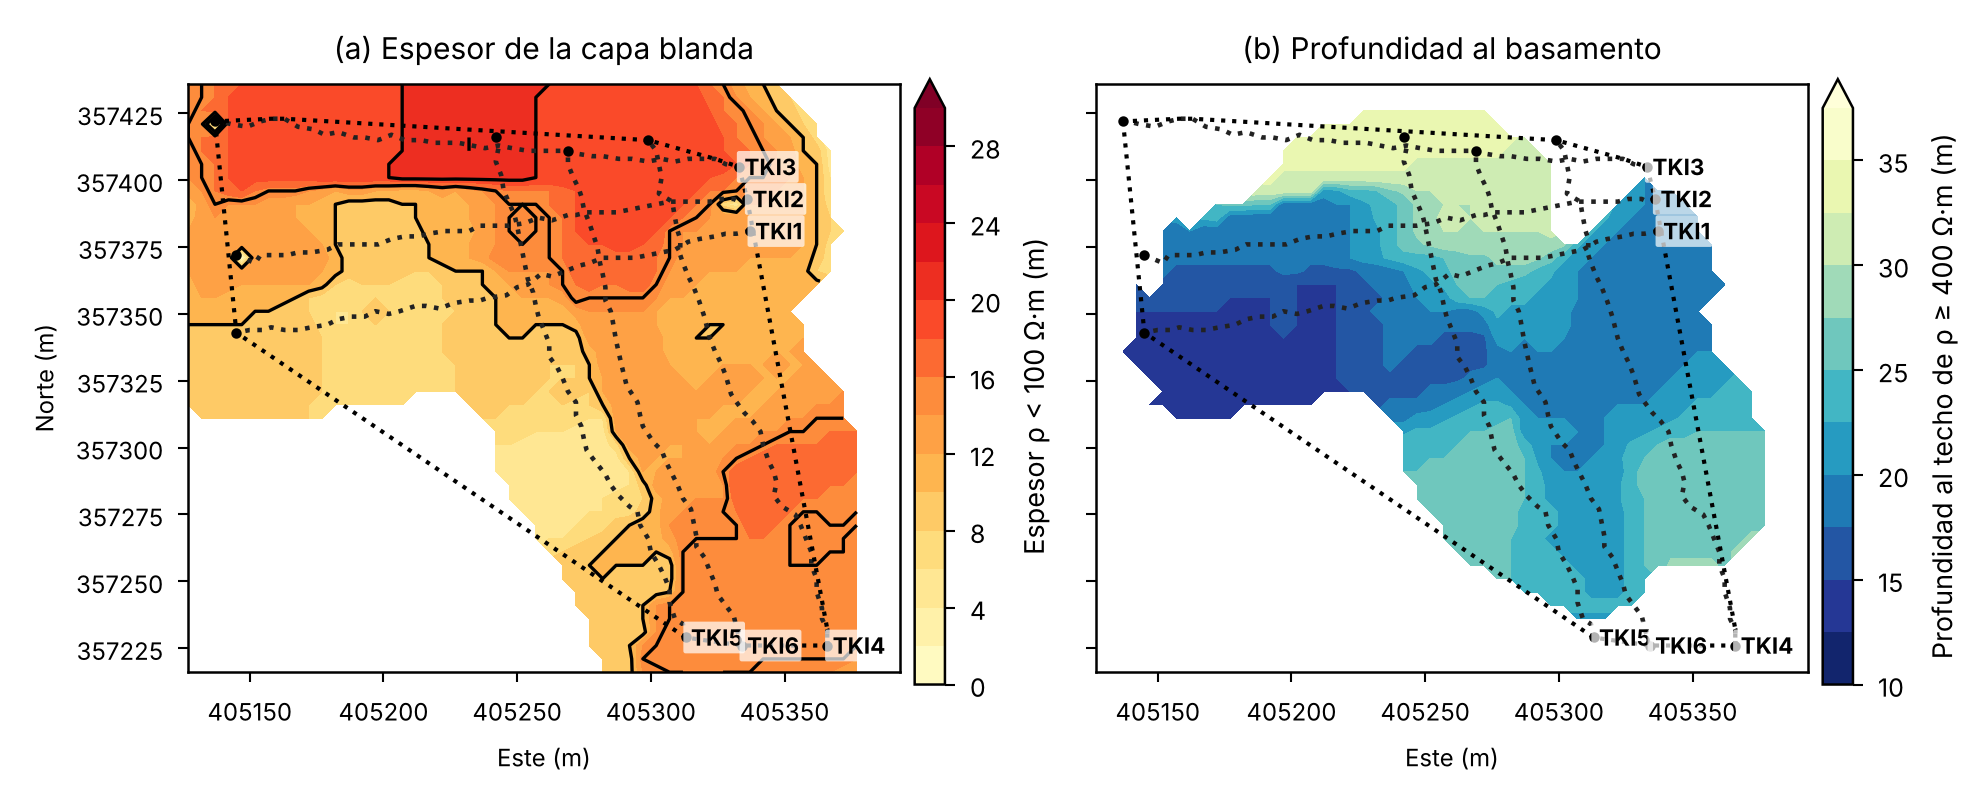
\includegraphics[width=0.94\textwidth]{p_espesor.png}
\caption{(a) Espesor de la capa blanda ($\rho<100$\,\ohmm; isolíneas de 10, 15 y 20\,m) y (b) profundidad al techo de $\rho\ge400$\,\ohmm. Cobertura limitada a 35\,m de algún perfil; línea punteada: envolvente de los perfiles.}
\label{fig:espesor}
\end{figure*}

La capa blanda alcanza 20\,m o más en el norte ($E\approx405\,220$--$405\,300$, $N\approx357\,385$--$357\,430$), de 14 a 18\,m en el noreste y el sureste, y menos de 8\,m en el centro-oeste ($E\approx405\,160$--$405\,270$, $N\approx357\,300$--$357\,370$). El basamento está a 10--15\,m en el oeste, a 22--27\,m en el sureste y a 30\,m o más en el norte, donde no se alcanza. Dentro de la envolvente de los perfiles (29\,275\,m\textsuperscript{2}), el volumen con $\rho<100$\,\ohmm{} es de $3.68\times10^{5}$\,\mcub{} (espesor medio de 12.7\,m), de los cuales $5.2\times10^{4}$\,\mcub{} corresponden al núcleo de $\rho<30$\,\ohmm. Con un margen de 15\,m alrededor de los perfiles, el volumen sube a $4.19\times10^{5}$\,\mcub, y a $5.30\times10^{5}$\,\mcub{} con 25\,m. El artículo reporta $3.12\times10^{5}$\,\mcub{} con un prisma rectangular \cite{arifin2020dib}. El valor obtenido aquí dentro de la envolvente es 18\,\% mayor. Si se usa un umbral de 70\,\ohmm{} en lugar de 100\,\ohmm{}, se obtiene $2.99\times10^{5}$\,\mcub, a 4\,\% del artículo. La diferencia depende, por lo tanto, del umbral y de la geometría del prisma, y no solo de los datos.

\textbf{Consistencia entre líneas.} Se compararon las columnas de resistividad en los nueve cruces entre las líneas E--O y N--S (Tabla~\ref{tab:cruces}). Donde la profundidad común supera 8\,m (seis cruces), el RMS de $\Delta\log_{10}\rho$ es de 0.08 a 0.24 (un factor de 1.2 a 1.75). Los cruces con TKI3 comparten solo de 1 a 3.5\,m de profundidad (el extremo norte de las líneas N--S tiene poca cobertura) y no son concluyentes.

\begin{table}[!t]
\caption{Consistencia en los cruces de líneas E--O (1--3) y N--S (4--6)}
\label{tab:cruces}
\centering
\small
\begin{tabular}{@{}ccccc@{}}
\toprule
Cruce & Dist. (m) & Prof. común (m) & RMS $\Delta\log_{10}\rho$ & Factor \\
\midrule
1--4 & 0.4 & 11.5 & 0.10 & 1.26 \\
1--5 & 0.6 & 17.5 & 0.10 & 1.25 \\
1--6 & 0.4 & 15.5 & 0.08 & 1.20 \\
2--4 & 0.0 & 8.5 & 0.24 & 1.75 \\
2--5 & 0.6 & 12.0 & 0.11 & 1.29 \\
2--6 & 0.3 & 11.0 & 0.14 & 1.37 \\
3--4 & 0.8 & 3.5 & 0.24 & 1.73 \\
3--5 & 0.3 & 2.5 & 0.18 & 1.51 \\
3--6 & 0.0 & 1.0 & 0.52 & 3.30 \\
\bottomrule
\end{tabular}
\end{table}

\subsection{Cargabilidad (IP)}
La cargabilidad del modelo va de 0 a 4.9\,ms (mediana de 2.0\,ms; percentiles 5--95: de 1.0 a 3.5\,ms), con un error de ajuste de 0.6 a 0.9\,ms. Por eso las diferencias menores que aproximadamente 1\,ms no son significativas (Fig.~\ref{fig:seisip}).

\begin{figure*}[!t]
\centering
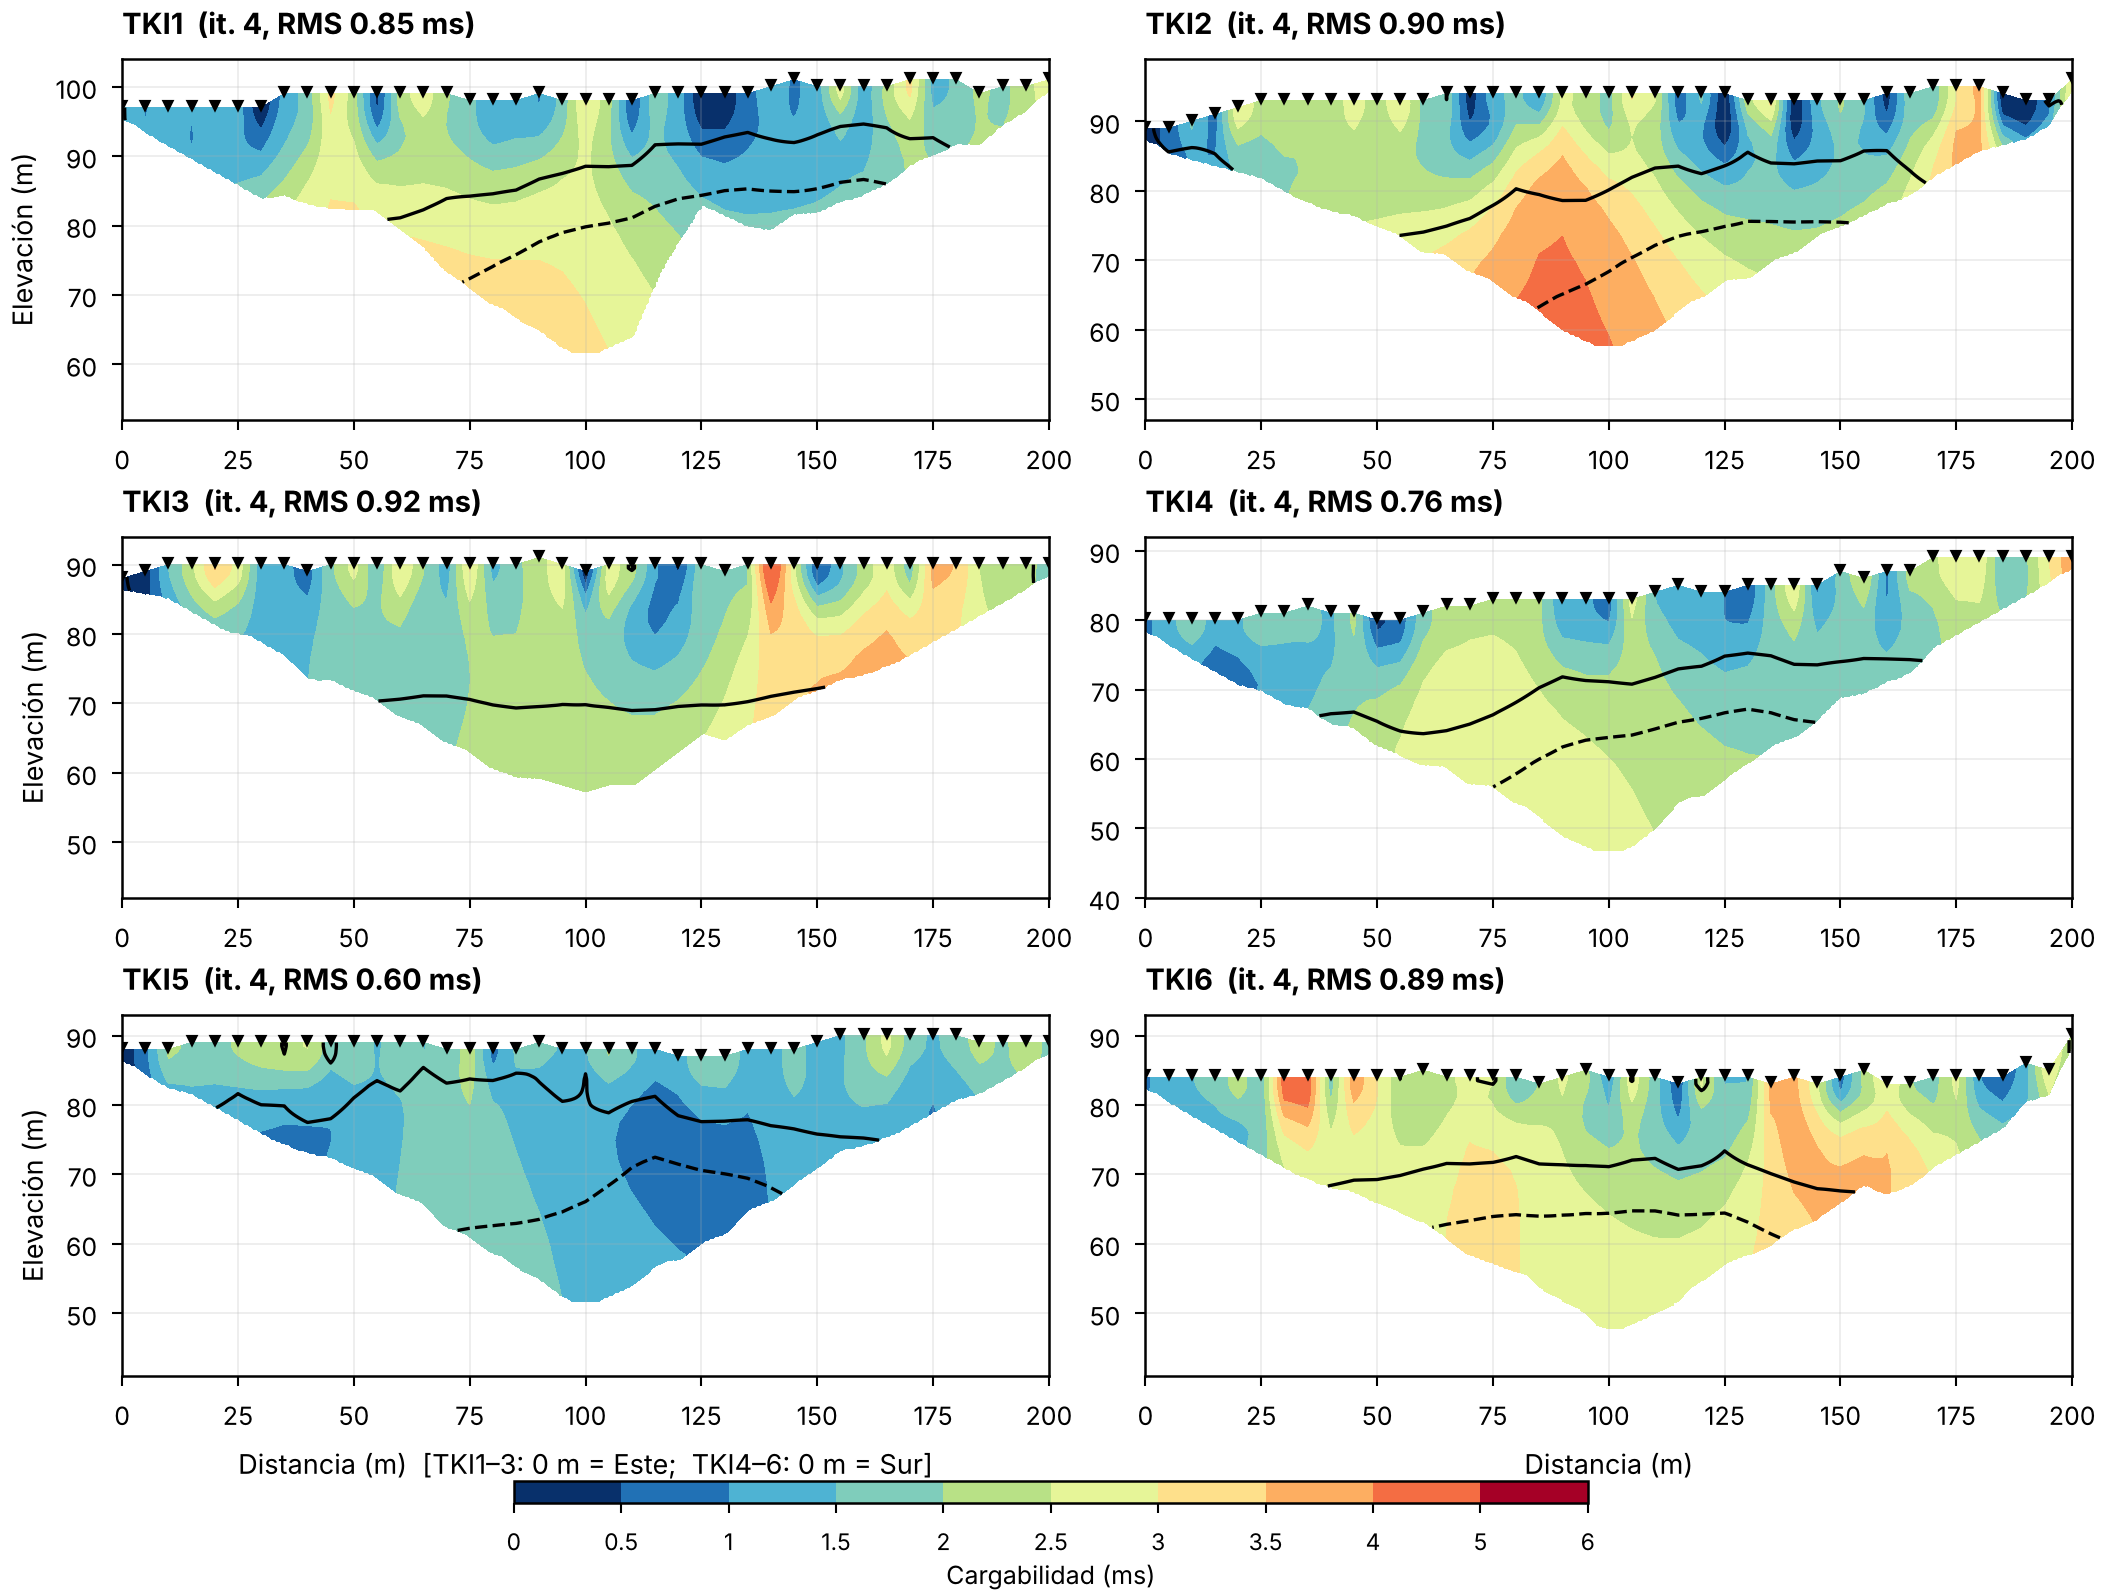
\includegraphics[width=\textwidth]{p_seis_ip.png}
\caption{Modelos de cargabilidad de las seis líneas (iteración 4 de resistividad, misma escala de 0 a 6\,ms). Se muestran las isolíneas de 100\,\ohmm{} (continua) y 400\,\ohmm{} (discontinua).}
\label{fig:seisip}
\end{figure*}

\textbf{Zonas de menor cargabilidad.} Los mínimos ($<1$\,ms) están sobre todo en la capa blanda somera. En TKI1, en $x=122$--137\,m (de 0 a 10\,m de profundidad, 0.6\,ms, $\rho$ mediana de 63\,\ohmm). En TKI2, en $x=121$--128, 139--144 y 184--195\,m (de 0 a 10\,m; 0.5 a 0.6\,ms; 37 a 46\,\ohmm). En TKI3, en $x=114$--121\,m (0.85\,ms; 38\,\ohmm). En TKI5, un cuerpo mayor (526\,m\textsuperscript{2}) con 0.9\,ms ocupa $x=107$--139\,m y de 4 a 28\,m de profundidad, con $\rho$ mediana de 380\,\ohmm. Es un volumen resistivo y poco polarizable, compatible con roca o saprolito (roca descompuesta) sin arcilla ni sulfuros. TKI4 y TKI6 no tienen zonas $<1$\,ms.

\textbf{Zonas de mayor cargabilidad.} Se distinguen dos grupos. (a) Profundos, en la clase consolidada y de basamento: TKI1 en $x=63$--104\,m y de 21 a 36\,m (3.1\,ms; 713\,\ohmm); TKI2 en $x=63$--120\,m y de 5 a 36\,m (3.6\,ms; 258\,\ohmm; 914\,m\textsuperscript{2}, el mayor); y TKI6 en $x=65$--80\,m y de 10 a 28\,m (3.1\,ms; 347\,\ohmm). (b) Someros, dentro de la capa blanda, con baja resistividad y alta cargabilidad: TKI2 en $x=170$--182\,m (3.4\,ms; 23\,\ohmm); TKI6 en $x=28$--37\,m (3.7\,ms; 25\,\ohmm) y en $x=132$--168\,m (3.4\,ms; 54\,\ohmm); y TKI3 en $x=137$--182\,m (3.4\,ms; 51\,\ohmm). Los del grupo (b) son los candidatos a residuos con finos arcillosos o fragmentos metálicos. El de TKI3 incluye la posición del electrodo 28 ($x=140$\,m), cuyos datos se eliminaron, y debe tomarse con reserva.

\textbf{Relación con la resistividad.} La resistividad y la cargabilidad no tienen una relación sistemática (Fig.~\ref{fig:rhoip}, Tabla~\ref{tab:ip}). Con las 2\,082 celdas del modelo, la correlación es $r=0.11$ (Spearman 0.06), y por línea $r$ va de $-0.31$ (TKI5) a $+0.30$ (TKI1). La cargabilidad media sube de 1.9 a 2.3\,ms de la capa blanda al basamento, un contraste menor que la dispersión (P10--P90 de 1.0 a 3.1\,ms) y que el error del modelo. En cambio, la cargabilidad normalizada $m/\rho$ \cite{slater2002}, un índice de la polarización relativa a la conductividad, es unas 13 veces mayor en la capa blanda (0.045) que en el basamento (0.0034). Esto se debe a que en la capa blanda se suman la conductividad de los iones y la polarización de las superficies (arcilla, finos del residuo). Con la resolución de la IP de este estudio, es un indicio y no una prueba.

\begin{figure*}[!t]
\centering
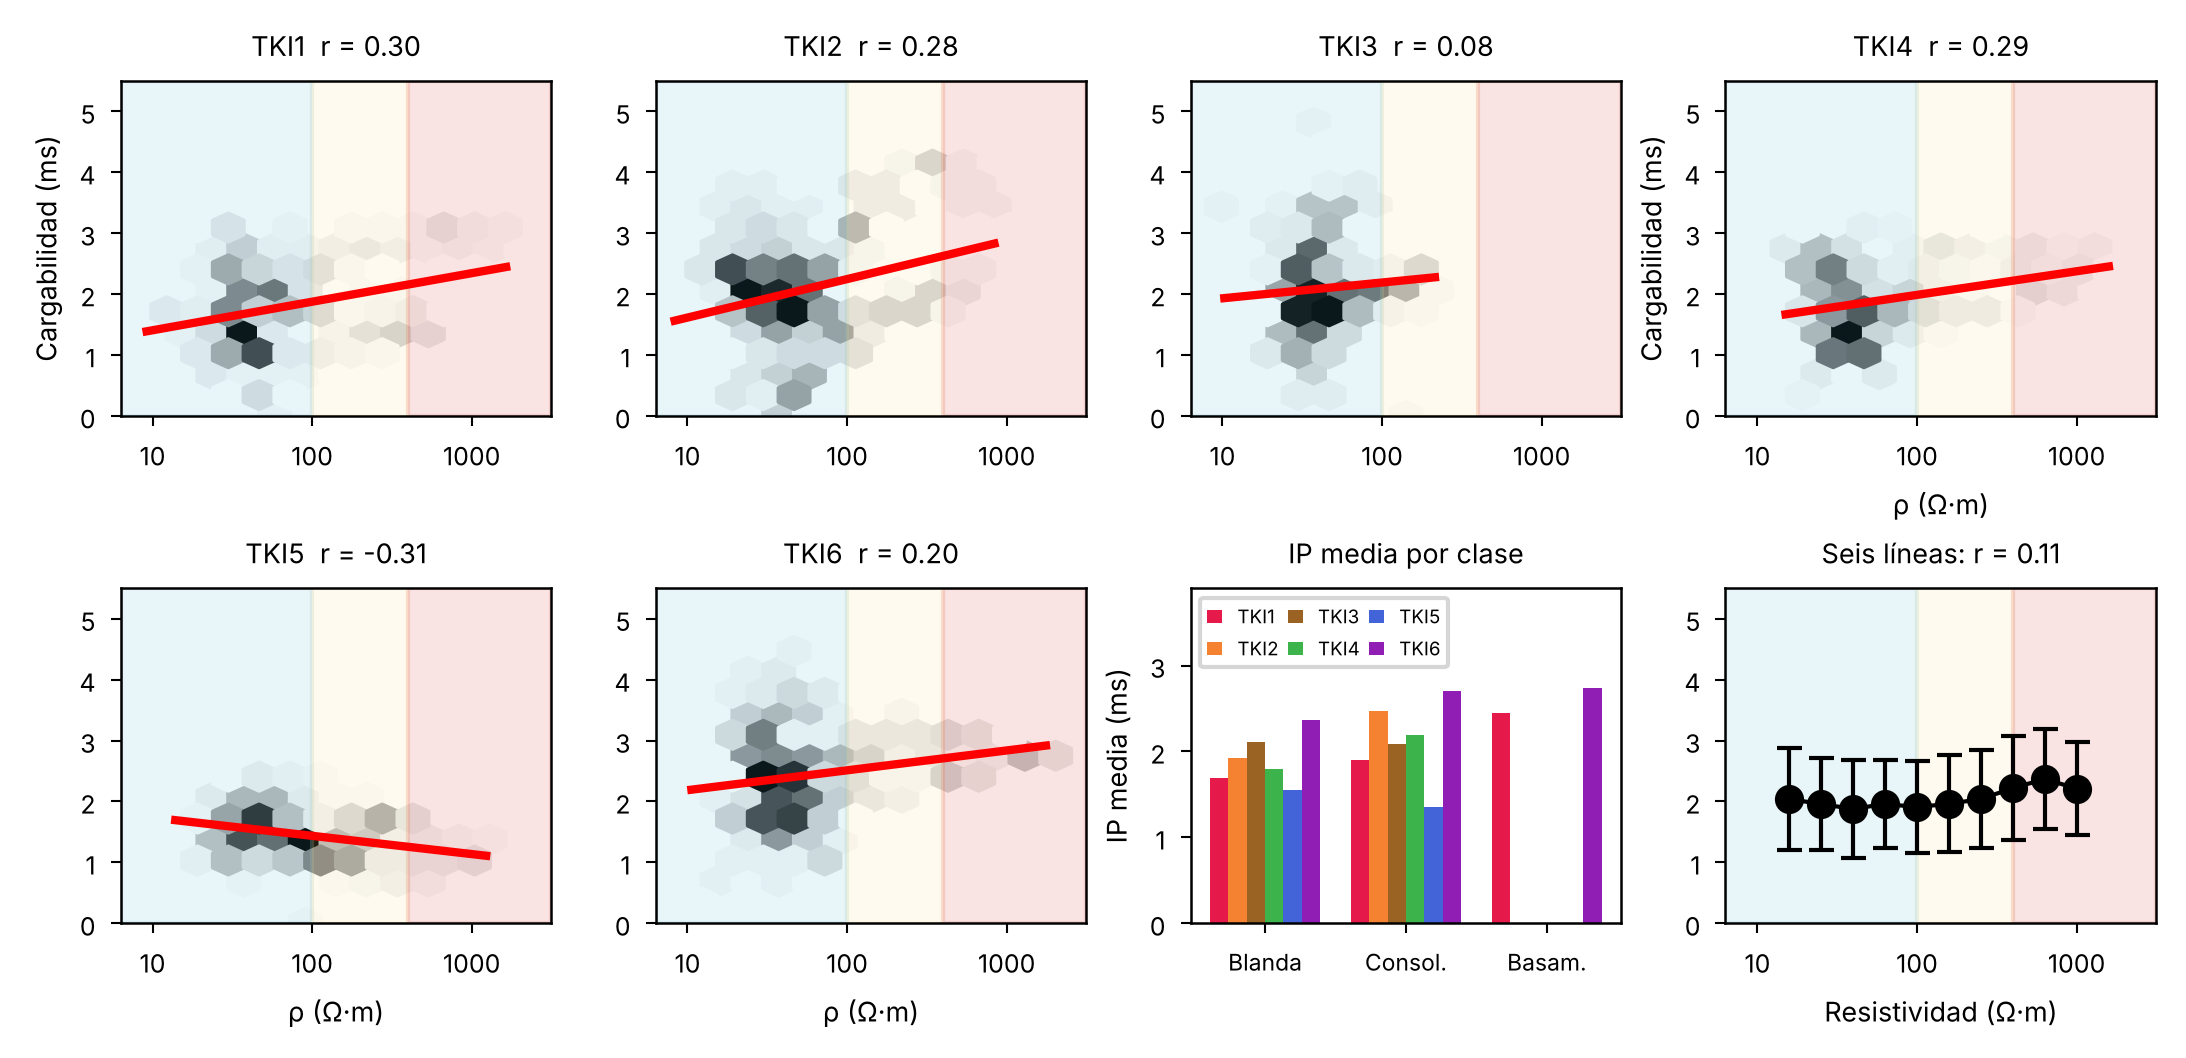
\includegraphics[width=\textwidth]{p_rho_ip.png}
\caption{Cargabilidad frente a resistividad en las celdas de los modelos invertidos (densidad de celdas en escala de grises; recta: ajuste lineal sobre $\log\rho$); media por clase y las seis líneas juntas (media $\pm$ desviación estándar por intervalo de resistividad). Franjas: azul, capa blanda; amarillo, consolidada; rojo, basamento.}
\label{fig:rhoip}
\end{figure*}

\begin{table*}[!t]
\caption{Cargabilidad esperada según la literatura y observada en el modelo}
\label{tab:ip}
\centering
\small
\begin{tabular}{@{}p{3.3cm}p{3.4cm}p{4.4cm}p{5.4cm}@{}}
\toprule
Material & $\rho$ esperada & IP esperada (literatura) & Observada: $\rho$ mediana; IP media (P10--P90) \\
\midrule
Lixiviado salino / residuo húmedo & muy baja ($<30$--80\,\ohmm) & baja a moderada (0.05--5.75\,ms en \cite{mepaiyeda2019}) & capa blanda: 39\,\ohmm; 1.9\,ms (1.0--2.9) \\
Residuo con arcilla o metal & baja & moderada a alta \cite{gazoty2012,slater2002} & zonas someras de 3.4--3.7\,ms con 23--54\,\ohmm \\
Roca consolidada / saprolito & 100--400\,\ohmm & baja a moderada & capa consolidada: 174\,\ohmm; 2.0\,ms (1.1--3.1) \\
Basamento sano & $>400$--1\,000\,\ohmm \cite{mepaiyeda2019} & baja & basamento: 663\,\ohmm; 2.3\,ms (1.1--3.1) \\
\bottomrule
\end{tabular}
\end{table*}

Los valores esperados de IP son cualitativos, porque dependen del instrumento, de la ventana de integración y de la definición de cargabilidad. Por eso los 0.05 a 5.75\,ms de \cite{mepaiyeda2019} no se pueden aplicar sin más a otro equipo. Aun así, el orden de magnitud observado (1 a 4\,ms) coincide con el de ese estudio de un relleno sanitario, donde los contaminantes tienen baja resistividad (34--80\,\ohmm) y baja cargabilidad, y el basamento tiene más de 1\,000\,\ohmm.

\subsection{Química de suelo y agua, y relación con la resistividad}
Las hojas de cálculo del artículo contienen tres muestras de suelo (KS-1 a KS-3) y tres de agua (KW1 a KW3) (Fig.~\ref{fig:quimica}). No indican las unidades, y se supusieron mg/kg para el suelo y \textmu g/L para el agua. El pH es neutro (6.7 a 7.3 en suelo; 7.0 a 7.2 en agua). En el agua dominan Ca, Mg, K y Na, y en el suelo Ca, Fe y Mg. Los metales pesados están solo en trazas (en el suelo: As 17--89, Cd 0.7--2.1, Cr 6--46, Cu 19--54, Pb 17--33, Ni 13--57, Zn 36--120\,mg/kg; Hg bajo el límite de detección).

\begin{figure*}[!t]
\centering
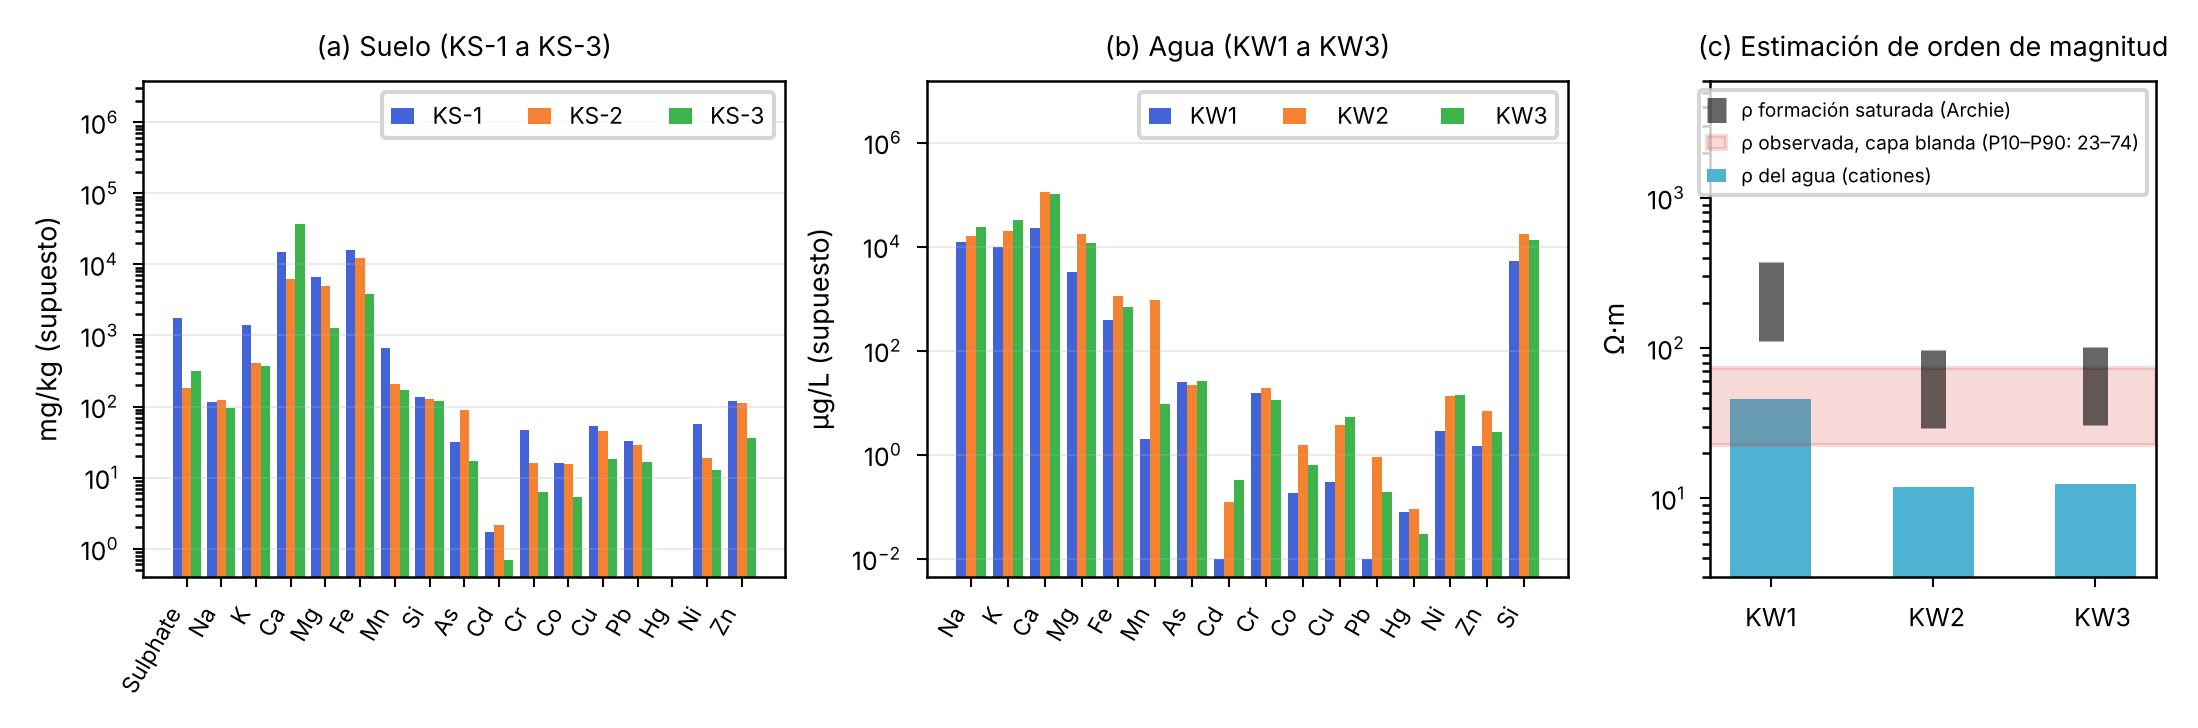
\includegraphics[width=\textwidth]{p_quimica.png}
\caption{Composición química (escala logarítmica) de (a) suelo y (b) agua, y (c) estimación de la resistividad del agua de poro a partir de cationes mayoritarios y de la formación saturada mediante la ley de Archie, frente a la resistividad observada en la capa blanda.}
\label{fig:quimica}
\end{figure*}

La literatura indica cómo afecta cada componente a las propiedades eléctricas:
\begin{itemize}
\item \textbf{Iones mayoritarios} (Na, K, Ca, Mg, Cl, SO$_4$, HCO$_3$): controlan la conductividad del fluido y, por la ley de Archie \cite{archie1942}, la resistividad: $\rho=\rho_w\,\phi^{-m}$, donde $\rho_w$ es la resistividad del agua, $\phi$ la porosidad y $m$ el factor de cementación. Los lixiviados salinos producen resistividades de decenas de \ohmm{} o menos \cite{aristodemou2000,mepaiyeda2019}.
\item \textbf{Metales pesados}: en concentraciones de \textmu g/L a mg/kg aportan una parte despreciable a la conductividad total. Sirven como indicadores de contaminación asociada a los residuos, no como causa de la anomalía eléctrica.
\item \textbf{Arcillas, óxidos de Fe y partículas metálicas}: aumentan la polarización. Las arcillas lo hacen por conducción en su superficie \cite{slater2002,gazoty2012}, y los metales y sulfuros, por polarización de electrodo.
\end{itemize}

Para comparar con los datos se estimó la conductividad eléctrica (CE) del agua con la regla empírica $\mathrm{CE}\,(\mu\mathrm{S/cm})\approx100\sum\text{cationes}\,(\mathrm{meq/L})$ \cite{hem1985}. Con 2.2, 8.4 y 8.0\,meq/L de cationes mayoritarios (KW1, KW2, KW3) resulta una CE de 219, 836 y 797\,\textmu S/cm y una $\rho_w$ de 46, 12 y 13\,\ohmm. Con $\phi=0.35$--0.50 y $m=1.3$--2.0, la formación saturada tendría 112--372\,\ohmm{} (KW1) y 29--102\,\ohmm{} (KW2 y KW3). El resultado, de orden de magnitud, es compatible con la capa blanda observada (P10--P90: 23 a 74\,\ohmm; mediana de 39). De aquí se sacan dos consecuencias. (1) La baja resistividad se explica por la humedad, por la mineralización moderada del agua de poro y por los finos del relleno, sin necesidad de metales pesados. (2) Una CE de 220 a 840\,\textmu S/cm es baja para un lixiviado concentrado (que suele ser de mS/cm), así que la capa blanda delimita el cuerpo de residuos y relleno húmedo, pero no necesariamente la pluma de mayor contaminación. Para eso se necesita muestreo a profundidad en los núcleos de $\rho<30$\,\ohmm.

\subsection{Comparación con un estudio previo en un relleno cercano}
Para tener con qué comparar, se revisó el informe de Umor y Arifin \cite{umor2011}, un estudio de 2011 en otro relleno de Kepong (Taman Nanyang, Wahyu y Delima). Por las coordenadas de su Tabla~1, está a unos 2.3--2.6\,km al este del sitio de este trabajo. Ese estudio solo midió resistividad: no tiene IP ni TEM. La Tabla~\ref{tab:comp2011} muestra en qué se parecen y en qué no.

\begin{table}[!t]
\caption{Comparación con el estudio de 2011}
\label{tab:comp2011}
\centering
\small
\setlength{\tabcolsep}{3pt}
\begin{tabular}{@{}p{1.65cm}p{2.85cm}p{3.2cm}@{}}
\toprule
 & 2011 (KPG01--05) & Este trabajo (TKI1--6) \\
\midrule
Medición & Resistividad & Resistividad e IP \\
Arreglo & Wenner & Wenner--Schlumberger \\
Líneas & 5 de 200\,m, 41 electrodos cada 5\,m, unos 30\,m de profundidad & 6 de 200\,m, 41 electrodos cada 5\,m, unos 35\,m de profundidad \\
RMS (\%) & 6.1 a 10.6 & 5.4 a 7.4 \\
$\rho$ del lixiviado & Texto: $<1$\,\ohmm; en KPG04, unos 6--27 (leyenda) & Mínimo de 8.3\,\ohmm; el 11.9\,\% de las celdas $<30$ \\
Sondeo & Uno (en KPG03) & Ninguno \\
Lixiviado visible & Charco y drenaje & Depresiones (Fig.~\ref{fig:fotos}) \\
\bottomrule
\end{tabular}
\end{table}

En el texto del estudio de 2011, el lixiviado (el líquido que escurre de los residuos) es lo que mide menos de 1\,\ohmm; de 1 a 10\,\ohmm{} es cubierta húmeda, y más de 10\,\ohmm{} (más de 30 en una línea), cubierta seca. Pero cada una de sus cinco secciones usa su propia escala de colores. En KPG04, la línea que más destacan, las zonas marcadas como lixiviado tienen colores que, según la leyenda de esa misma figura, equivalen a unos 6 a 27\,\ohmm, con un centro por debajo de unos 6\,\ohmm{} (Fig.~\ref{fig:secc2011}a). O sea, el límite que escriben no coincide con lo que dibujan. Además, su clasificación se apoya en un solo sondeo: encontró madera gris y café (señal de residuos) entre 6 y 6.45\,m y no recuperó material entre 7.0 y 13.9\,m. Los propios autores dicen que hay un solo sondeo.

\begin{figure*}[!t]
\centering
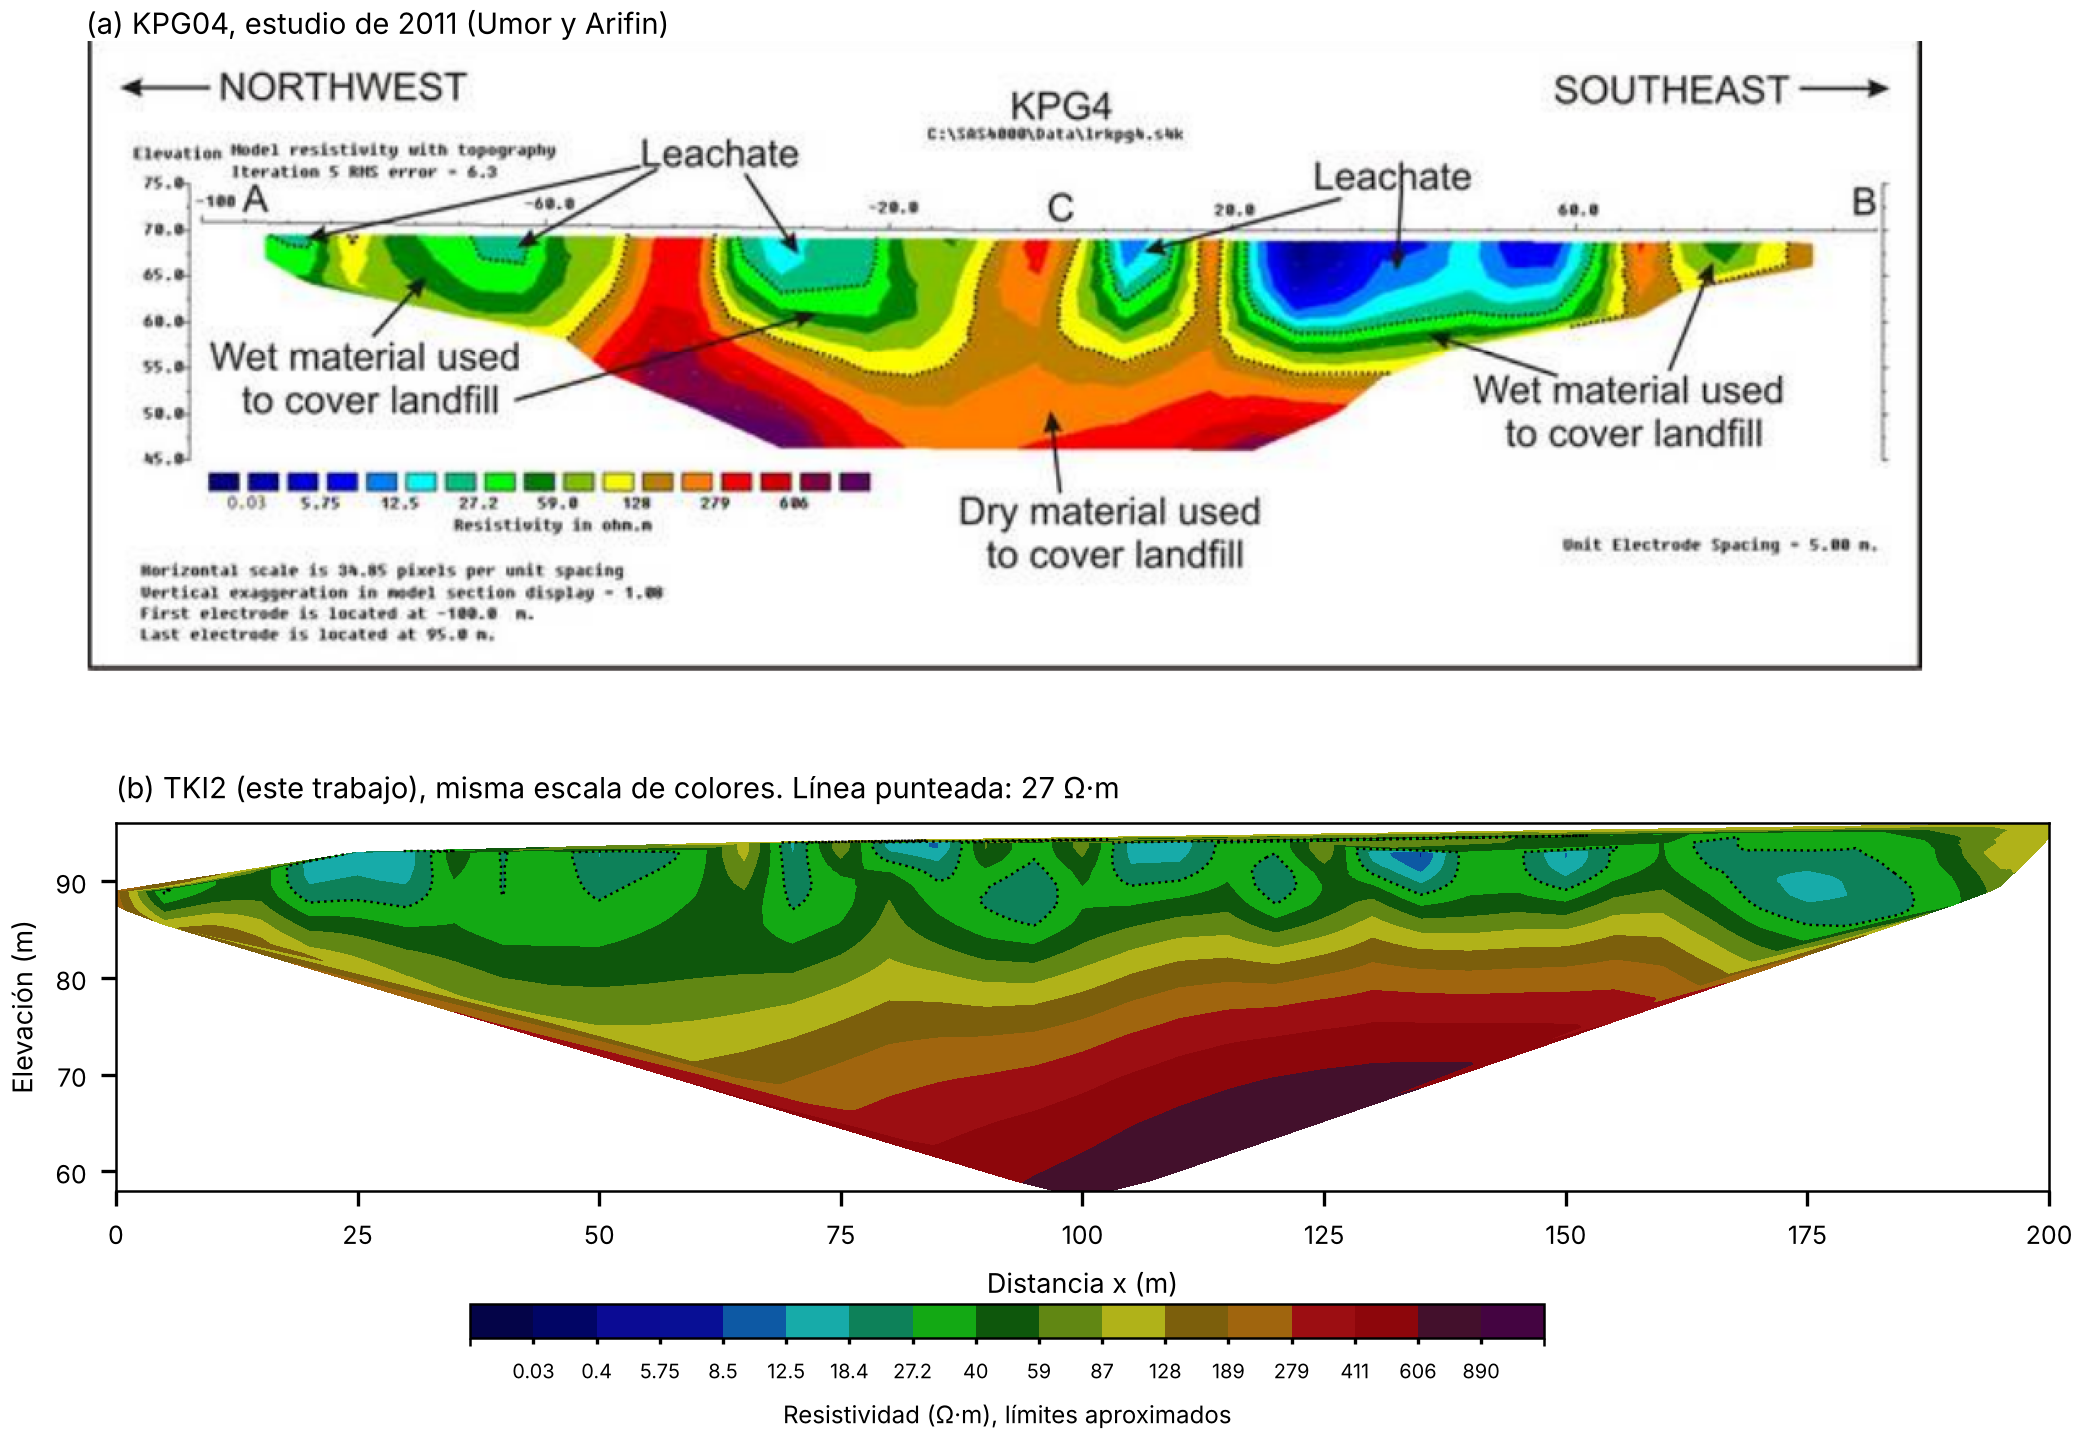
\includegraphics[width=0.93\textwidth]{p_secc2011.png}
\caption{(a) Sección KPG04 del estudio de 2011, recortada de \cite{umor2011}. (b) Sección TKI2 de este trabajo dibujada con la misma escala de colores. Los límites entre colores se leyeron de la leyenda de KPG04 y se interpolaron, así que son aproximados.}
\label{fig:secc2011}
\end{figure*}

Con la misma escala (Fig.~\ref{fig:secc2011}b), la parte superficial de TKI2 tiene zonas de 12 a 27\,\ohmm{} (colores cian y verde azulado) parecidas en color y tamaño a algunas que en 2011 se llamaron lixiviado. No hay zonas en azul oscuro (menos de unos 6\,\ohmm). En TKI2, el 11.4\,\% de las celdas está por debajo de 27.2\,\ohmm.

\begin{figure*}[!t]
\centering
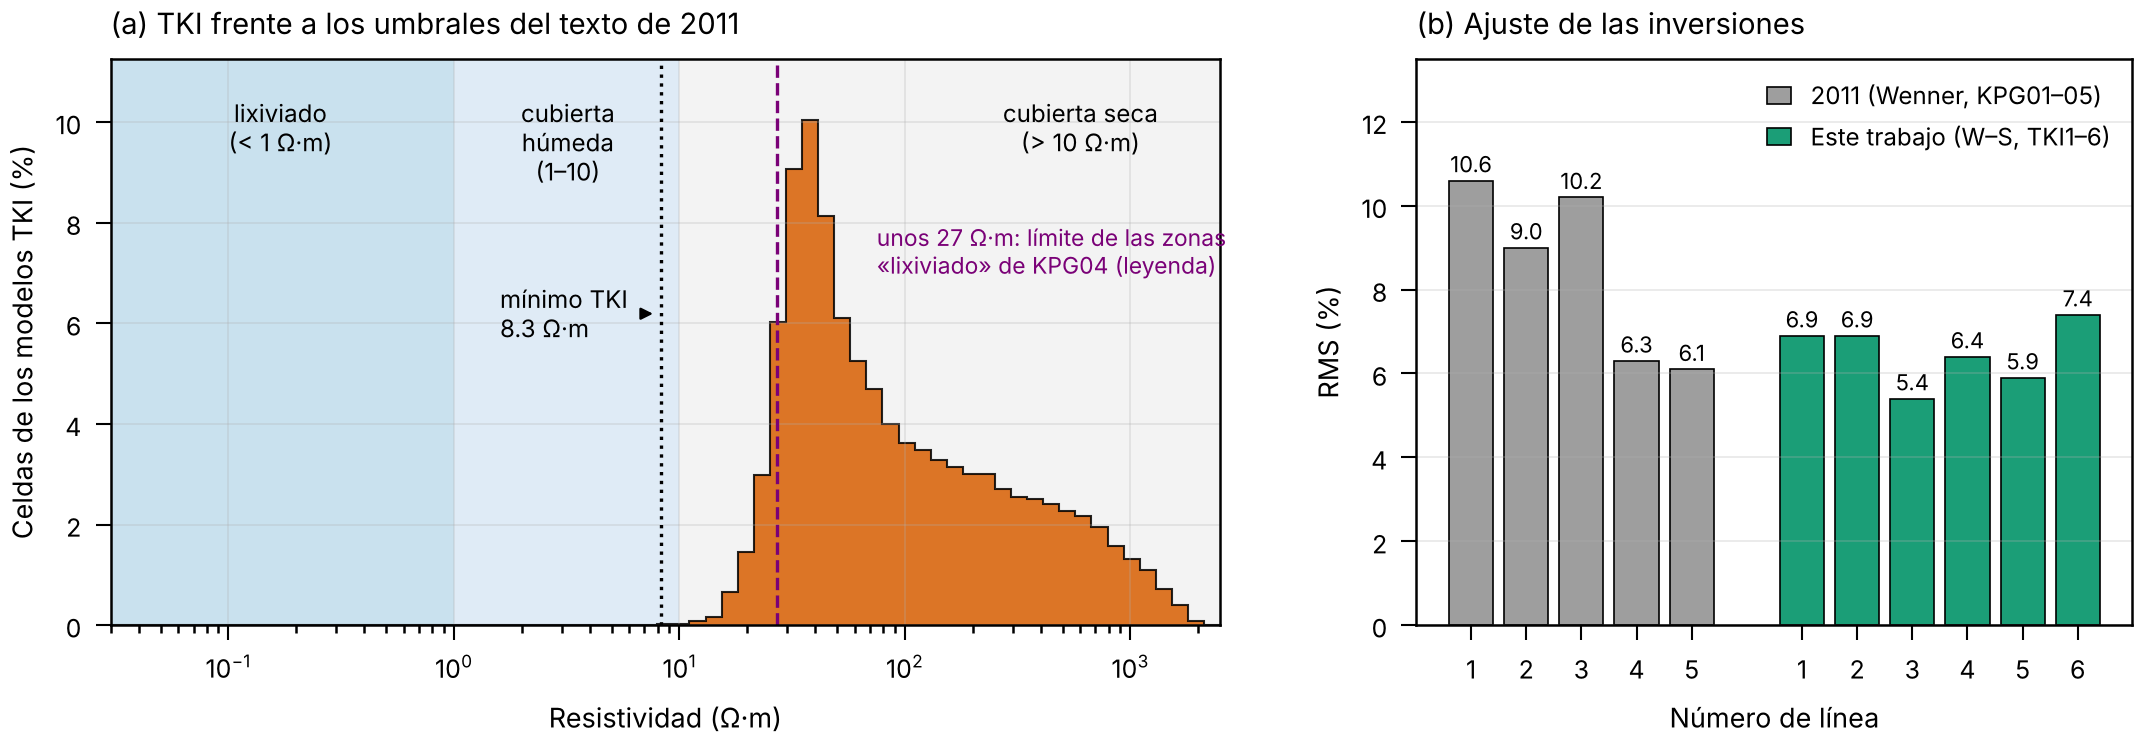
\includegraphics[width=\textwidth]{p_comp2011.png}
\caption{(a) Distribución de la resistividad de las 45\,750 celdas de los modelos TKI frente a los umbrales del texto de 2011 y al límite de unos 27\,\ohmm{} leído en KPG04. (b) RMS de las inversiones de ambos estudios; los programas, los arreglos y la edición de datos son distintos, así que la comparación es solo orientativa.}
\label{fig:comp2011}
\end{figure*}

La Fig.~\ref{fig:comp2011}a lo resume: ninguna celda de los modelos TKI baja de 8.3\,\ohmm{} y solo el 0.02\,\% está por debajo de 10\,\ohmm, pero el 11.9\,\% está por debajo de 30\,\ohmm. Por eso los límites de 2011 no se pueden usar tal cual en TKI: cambian de un sitio y de una línea a otra, y casi no tienen sondeos que los respalden. El ajuste de las inversiones (RMS) es parecido o mejor en TKI, de 5.4 a 7.4\,\%, frente a 6.1 a 10.6\,\% en 2011 (Fig.~\ref{fig:comp2011}b).

Para tener un criterio con base física se usó la ley de Archie, con los mismos valores de porosidad y cementación de la sección anterior ($\phi=0.35$--0.50 y $m=1.3$--2.0). Con ella se calculó qué resistividad tendría el terreno saturado según la conductividad eléctrica (CE) del agua (Tabla~\ref{tab:archie}). Los datos de otros rellenos de Malasia vienen de \cite{ahmed2001,hamzah2014}.

\begin{table}[!t]
\caption{Conductividad del agua y resistividad esperada de la formación (Archie)}
\label{tab:archie}
\centering
\small
\setlength{\tabcolsep}{3pt}
\begin{tabular}{@{}p{3.6cm}p{1.6cm}p{2.0cm}@{}}
\toprule
Agua & CE (mS/cm) & $\rho$ formación (\ohmm) \\
\midrule
Seri Petaling, pozo aguas arriba \cite{ahmed2001} & 0.11 & 224--742 \\
Seri Petaling, río \cite{ahmed2001} & 0.41 & 60--199 \\
KW1 a KW3 (este trabajo, estimada) & 0.22--0.84 & 29--373 \\
Capa blanda de TKI (CE que la explicaría) & 0.3--3.6 & 23--74 \\
Seri Petaling, pozo aguas abajo \cite{ahmed2001} & 7.16 & 3.4--11.4 \\
Sungai Sedu \cite{hamzah2014} (según su resumen) & 6.6 a 50 & 0.5--12.4 \\
\bottomrule
\end{tabular}
\end{table}

La tabla se puede leer de tres maneras. (1) El agua de las muestras KW tiene una CE parecida a la del río de Seri Petaling y mucho menor que la de su agua contaminada. (2) Aun así, una capa blanda de 23 a 74\,\ohmm{} también se explicaría con agua de hasta unos 3.6\,mS/cm si la porosidad es baja. Con solo tres muestras no se puede descartar agua moderadamente afectada en los núcleos de menos de 30\,\ohmm. (3) Un agua tan salina como la contaminada de Seri Petaling o Sungai Sedu daría menos de unos 12\,\ohmm, y eso no aparece en los modelos TKI. En Seri Petaling, además, los residuos saturados con lixiviado midieron de 6 a 7\,\ohmm{} en laboratorio, y los saturados con agua de lluvia, de 20 a 22.5\,\ohmm \cite{ahmed2001}.

En resumen, en el relleno de 2011 el lixiviado se dibujó con colores de unos 6 a 27\,\ohmm, y TKI tiene zonas superficiales en ese mismo rango. Lo que no aparece en TKI es la señal de un agua muy salina (menos de unos 12\,\ohmm). Los datos apoyan que hay zonas afectadas por humedad y agua de salinidad moderada, además del lixiviado visible en superficie, pero no bastan para afirmar que exista una pluma concentrada en profundidad. Tampoco la descartan: en Sungai Sedu \cite{hamzah2014}, en residuos viejos el modelo dio 100 a 200\,\ohmm{} y la medición dentro del pozo dio 30 a 40\,\ohmm, o sea que una inversión suavizada puede mostrar valores más altos que los reales. Para decidirlo hacen falta pozos y muestras de agua en los núcleos de menos de 30\,\ohmm.

\section{Limitaciones}
Los resultados dependen de varias decisiones y supuestos que conviene tener presentes:
\begin{itemize}
\item La inversión usa un código propio y no RES2DINV, así que las cifras pueden diferir un poco.
\item Las cotas \gps{} difieren hasta 14\,m entre líneas que se cruzan, lo que obligó a interpolar en profundidad. La incertidumbre horizontal de las celdas interpoladas es del orden de 5\,m.
\item La resolución baja con la profundidad y en los extremos de las secciones. El techo del basamento y las zonas de mayor cargabilidad en el extremo de las líneas son menos confiables.
\item Las clases por resistividad no se calibraron con sondeos ni con la geología local; su relación con tipos de roca es una hipótesis.
\item Retirar el electrodo 28 reduce la cobertura en $x\approx120$--$145$\,m en todas las líneas.
\item El contraste de IP después de la edición es pequeño (0.5 a 5\,ms) comparado con el que reporta el artículo para sus modelos.
\item Las unidades de la química se supusieron, y las muestras (tres de suelo y tres de agua) son pocas.
\item La comparación con el estudio de 2011 es solo orientativa: es otro relleno, con otro arreglo y otro programa de inversión, y su clasificación tiene un solo sondeo. Los límites de color de su leyenda se leyeron de una imagen, así que son aproximados.
\end{itemize}

\section{Conclusiones}
\begin{enumerate}
\item Con la topografía incluida y la iteración 4 se obtuvieron modelos con RMS de 5.4 a 7.4\,\%, cuyas resistividades (de 8 a 2\,040\,\ohmm) son del orden de las clases del artículo (hasta 2\,000\,\ohmm).
\item La capa blanda ($<100$\,\ohmm) tiene su base media a 8--19\,m y ocupa de 43 a 82\,\% de cada sección. El techo del basamento ($>400$\,\ohmm) está a 14--31\,m, salvo en TKI3, donde no se alcanza.
\item El modelo 3D indica un volumen de $3.7\times10^{5}$\,\mcub{} con $\rho<100$\,\ohmm, con el mayor espesor al norte (más de 20\,m) y el menor en el centro-oeste (menos de 8\,m). El artículo da $3.12\times10^{5}$\,\mcub, y la diferencia depende del umbral y de la geometría.
\item La cargabilidad (0.5--5\,ms) no se relaciona de forma consistente con la resistividad ($r=0.11$) ni distingue las clases. Su mayor utilidad es señalar zonas someras, conductoras y polarizables, como candidatas a residuos con finos o metal.
\item La baja resistividad de la capa blanda es coherente con la mineralización moderada del agua de poro (CE estimada de 220 a 840\,\textmu S/cm) y no exige metales pesados. Identificar la pluma contaminada requiere muestreo dirigido a los núcleos de $\rho<30$\,\ohmm.
\item Frente al relleno cercano de 2011 \cite{umor2011}, donde el lixiviado se dibujó con colores de unos 6 a 27\,\ohmm, TKI tiene zonas superficiales de esa magnitud (el 11.9\,\% de las celdas está por debajo de 30\,\ohmm), pero ninguna celda baja de 8.3\,\ohmm y la CE de las muestras es baja (0.22 a 0.84\,mS/cm). Los datos apoyan zonas afectadas por humedad y salinidad moderada, no una pluma muy salina.
\end{enumerate}

\begin{thebibliography}{99}
\bibitem{aristodemou2000} E. Aristodemou y A. Thomas-Betts, ``DC resistivity and induced polarisation investigations at a waste disposal site and its environs,'' \textit{J. Appl. Geophys.}, vol. 44, n.º 2--3, pp. 275--302, 2000.
\bibitem{gazoty2012} A. Gazoty, G. Fiandaca, J. Pedersen, E. Auken, A. V. Christiansen y J. K. Pedersen, ``Application of time domain induced polarization to the mapping of lithotypes in a landfill site,'' \textit{Hydrol. Earth Syst. Sci.}, vol. 16, n.º 6, pp. 1793--1804, 2012.
\bibitem{mepaiyeda2019} S. Mepaiyeda, K. Madi, O. Gwavava, C. Baiyegunhi y L. Sigabi, ``Contaminant delineation of a landfill site using electrical resistivity and induced polarization methods in Alice, Eastern Cape, South Africa,'' \textit{Int. J. Geophys.}, vol. 2019, art. 5057832, 2019.
\bibitem{arifin2020dib} M. H. Arifin, J. S. Kayode, K. I. Ismail, M. Abdullah, A. Embrandiri, S. M. Nazer y A. Azmi, ``Data for the industrial and municipal environmental wastes hazard contaminants assessment with integration of RES2D techniques and Oasis Montaj software,'' \textit{Data in Brief}, vol. 33, art. 106595, 2020. doi:10.1016/j.dib.2020.106595.
\bibitem{tan1977} B. K. Tan y E. B. Yeap, ``Structure of the Kenny Hill Formation, Kuala Lumpur and Selangor,'' \textit{Bull. Geol. Soc. Malaysia}, vol. 8, pp. 127--129, 1977.
\bibitem{filipov2021} A. Filipov, J. Jong y M. Madon, ``Reconnaissance of Kenny Hill Formation outcrops in the Rawang area, northern Selangor, Malaysia,'' \textit{Warta Geologi}, vol. 47, n.º 1, pp. 29--48, 2021.
\bibitem{dey1979} A. Dey y H. F. Morrison, ``Resistivity modelling for arbitrarily shaped two-dimensional structures,'' \textit{Geophys. Prospect.}, vol. 27, n.º 1, pp. 106--136, 1979.
\bibitem{degroot1990} C. deGroot-Hedlin y S. Constable, ``Occam's inversion to generate smooth, two-dimensional models from magnetotelluric data,'' \textit{Geophysics}, vol. 55, n.º 12, pp. 1613--1624, 1990.
\bibitem{loke1996} M. H. Loke y R. D. Barker, ``Rapid least-squares inversion of apparent resistivity pseudosections by a quasi-Newton method,'' \textit{Geophys. Prospect.}, vol. 44, n.º 1, pp. 131--152, 1996.
\bibitem{loke2016} M. H. Loke, ``Tutorial: 2-D and 3-D electrical imaging surveys,'' Geotomo Software, 2016. [En línea]. Disponible: \url{http://www.geotomosoft.com}
\bibitem{seigel1959} H. O. Seigel, ``Mathematical formulation and type curves for induced polarization,'' \textit{Geophysics}, vol. 24, n.º 3, pp. 547--565, 1959.
\bibitem{oldenburg1994} D. W. Oldenburg y Y. Li, ``Inversion of induced polarization data,'' \textit{Geophysics}, vol. 59, n.º 9, pp. 1327--1341, 1994.
\bibitem{slater2002} L. D. Slater y D. Lesmes, ``IP interpretation in environmental investigations,'' \textit{Geophysics}, vol. 67, n.º 1, pp. 77--88, 2002.
\bibitem{archie1942} G. E. Archie, ``The electrical resistivity log as an aid in determining some reservoir characteristics,'' \textit{Trans. AIME}, vol. 146, pp. 54--62, 1942.
\bibitem{hem1985} J. D. Hem, ``Study and interpretation of the chemical characteristics of natural water,'' U.S. Geological Survey, Water-Supply Paper 2254, 3.\textsuperscript{a} ed., 1985.
\bibitem{umor2011} M. R. Umor y M. H. Arifin, ``Geoelectrical resistivity survey at landfill treatment near Taman Nanyang, Wahyu and Delima, Kepong, Selangor,'' informe técnico para Kumpulan IKRAM Sdn. Bhd. y JKR Cawangan Kejuruteraan Cerun, Universiti Kebangsaan Malaysia, nov. 2011.
\bibitem{ahmed2001} A. M. Ahmed y W. N. Sulaiman, ``Evaluation of groundwater and soil pollution in a landfill area using electrical resistivity imaging survey,'' \textit{Environ. Manage.}, vol. 28, n.º 5, pp. 655--663, 2001.
\bibitem{hamzah2014} U. Hamzah, M. Jeeva y N. A. M. Ali, ``Electrical resistivity techniques and chemical analysis in the study of leachate migration at Sungai Sedu landfill,'' \textit{Asian J. Appl. Sci.}, vol. 7, n.º 7, pp. 518--535, 2014. doi:10.3923/ajaps.2014.518.535.
\end{thebibliography}

\end{document}
